\documentclass{kththesis}
\usepackage{csquotes} % Recommended by biblatex
\usepackage[style=numeric,sorting=none,backend=biber]{biblatex}
\usepackage{amssymb}
\usepackage{hyperref}
\usepackage{amsthm}
\usepackage{amsmath}
\usepackage{mathtools}
\usepackage{listings}
\usepackage{minted}
\usepackage{tcolorbox}
\usepackage{color}
\usepackage{mips}

\usepackage{etoolbox} 


%\DeclareFieldFormat{urldate}{
%    (Accessed \thefield{urlyear}-\thefield{urlmonth}-\thefield{urlday}\isdot)}

\newtheorem*{definition}{Definition}

%T: Set up toc links
\hypersetup{
    linktoc=all,     %set to all if you want both sections and subsections linked
    linkcolor=black,  %choose some color if you want links to stand out
}

\addbibresource{references.bib} % The file containing our references, in BibTeX format

\title{Alternating Control Flow Graph Reconstruction by Combining Constant Propagation and Strided Intervals with Directed Symbolic Execution}
\alttitle{Alternaterande kontrollflödesgrafsrekonstruktion genom att kombinera propagerande av konstanter och klivande intervaller med riktad symbolisk exekvering }
\author{Thomas Peterson}
\email{thpeter@kth.se}
\supervisor{Roberto Guanciale} 
\examiner{Mads Dam}
\programme{Master in Computer Science}
\school{School of Electrical Engineering and Computer Science}
\date{\today}

%-----Custom Commands-----
\newcommand{\MONTH}{%
  \ifcase\the\month
  \or January % 1
  \or February % 2
  \or March % 3
  \or April % 4
  \or May % 5
  \or June % 6
  \or July % 7
  \or August % 8
  \or September % 9
  \or October % 10
  \or November % 11
  \or December % 12
  \fi}
  
\renewcommand{\it}[1]{\textit{#1}}

\renewcommand\fcolorbox[4][]{\textcolor{cyan}{\strut#4}} %Remove minted error boxes


%TODO: avoid using linespread, instead see ans two of https://tex.stackexchange.com/questions/30516/how-to-avoid-background-frame-break-in-code-listings-with-math-mathescape
\lstdefinestyle{frame}{
        columns=fullflexible,
        frame=single,
        mathescape=true,
        tabsize=4,
}

\lstdefinestyle{abstractInt}{
        aboveskip=1.4em,
        basicstyle=\linespread{2}\ttfamily\small,
        belowskip=0em,
        columns=fullflexible,
        frame=single,
        mathescape=true,
        tabsize=4,
}

\lstdefinestyle{algorithm}{
    basicstyle=\linespread{1.2}\small,
    columns=fullflexible,
    emph={Input,Output,if,else,foreach,for,while,return},
    emphstyle=\textbf,
    frame=single,
    mathescape=true,
    tabsize=4,
}

\lstdefinestyle{top}{
  abovecaptionskip=-1pt
  float=tp,
  floatplacement=tbp,
}

% Uncomment the next line to include cover generated at https://intra.kth.se/kth-cover?l=en
% \kthcover{kth-cover.pdf}


%---Notes---
%A conscientiously written scientific report in Swedish or English where the problem is introduced, different methods for the solution are discussed, the method chosen is presented, the solution and the results are described and the results are analyzed

%---Before Handing in the Report--
%Check if roman numbering should include list of tables/figures

%Content checklist: https://www.kth.se/social/group/examensarbete-vid-cs/page/degree-project-checklist/

%Formalitiees checklist: https://www.kth.se/social/group/examensarbete-vid-cs/page/formalities-checklist/

%Read the opposition documents: https://www.kth.se/social/group/examensarbete-vid-cs/page/public-discussion-and-examination/

%Check that all sources look good! And try to double check correctness!
%---------------------------------
%---TODO---
%Ensure abbreviations(like CFG) are introduced with the first occurrence of the notion
%Ensure consistent usage of intel or AT&T x86 syntax
%---------------------------------
%---Potential things to add---
% Info on stripped vs non-stripped binaries
% Lattice background?
%---------------------------------

\begin{document}

% Frontmatter includes the titlepage, abstracts and table-of-contents
\frontmatter

\titlepage

\begin{abstract}
%\\ \\
%\textbf{Keywords}\\
%Binary analysis, Control flow reconstruction, concolic execution
\end{abstract}


\begin{otherlanguage}{swedish}
  \begin{abstract}
    ...
  \end{abstract}
\end{otherlanguage}
%\clearpage
%\section*{Acknowledgement}
%I would like to thank my supervisor Roberto Guanciale, for his feedback and guiding throughout the research and writing of this report. 
%\\ \\
%Thank you! 
%\\ \\ \\ \\
%Stockholm, \MONTH \the\year
%\\ \\
%\it{Thomas Peterson}

\tableofcontents
\thispagestyle{empty}

\clearpage
\thispagestyle{empty}
\section*{Abbreviations}
\textbf{BBG:} Basic Block Graph\\
\textbf{CFG:} Control Flow Graph\\
\textbf{CFA:} Control Flow automaton\\
\textbf{IR:} Intermediate Representation\\
\textbf{Jakstab:} \textbf{Ja}va tool\textbf{k}it for \textbf{sta}tic analysis of \textbf{b}inaries\\

\clearpage
\thispagestyle{empty}
\section*{Glossary}
\textbf{Direct Jump:} A jump instruction which jumps to an explicit address.\\
\textbf{CFG:} A BBG or a CFA.\\
\textbf{Indirect Jump:} A jump instruction which jumps to an address located in a register or a memory location.\\
\textbf{Jump table:} A data structure which sometimes results from switch cases and leads to indirect jumps. \\
%\textbf{Transpilation:} The act of translating a binary program into its equivalent IL program\\

\listoffigures
\thispagestyle{empty}
 
\listoftables
\thispagestyle{empty}

% Mainmatter is where the actual contents of the thesis goes
\mainmatter
\cleardoublepage
\pagenumbering{arabic}

%---INFO ABOUT CITATIONS---
%We use the \emph{biblatex} package to handle our references.  We therefore use the command \texttt{parencite} to get a reference in parenthesis, like this \parencite{heisenberg2015}.  It is also possible to include the author as part of the sentence using \texttt{textcite}, like talking about the work of \textcite{einstein2016}.

\chapter{Introduction}
%X The question is easy to identify, the project's purpose and objective are clear.
%X The problem (and the student's contribution) has defined limits, its relevance is justified and put in context
%
%Explain why we want to study the binary instead of the source code. Use example in WYSINWYX where memset was removed by compiler?
Software is normally not developed directly in machine code but indirectly in a higher-level programming language such as C. Before a program can be used, its code must be compiled into architecture-dependent machine code. However, the compilation process can vary depending on many factors such as, for example, the type of compiler and the optimization level. Thus, software written in a non-assembly language might have multiple binary representations, some of which might even be erroneous\cite{preciseCFG}. Thus, when analysing software, it might be incorrect to expect properties which hold in the source code to hold in the compiled binary. A prime example of this is XcodeGhost.
\\ \\
Xcode is an application development framework for building IOS applications, developed by Apple\cite{Xcode}. In china, network speeds to apple's servers could sometimes be very slow and IOS developers thus commonly shared copies of Xcode installers through alternative hosting services\cite{XcodeGhost}. In mid-2015, malicious copys of xcode installers began circulating. These installers, known as XcodeGhost\cite{XcodeGhost}, appeared to behave identically to the legitimate framework. However, during compile time, the framework would inject malware into the application. Thus, the developers working with the infected framework would unintentionally create infected applications. 
\\ \\
XcodeGhost was the first compiler malware in OS X and the first instance of the IOS App Store deploying a large amount of trojanized applications\cite{XcodeGhost}\cite{XcodeGhostFireEye}. It successfully infected a large amount of IOS applications, of which only two were immediately confirmed to succesfully have passed apples code review and been submitted to the App Store for public download\cite{XcodeGhost}. Later, the cyber sercurity company FireEye conducted an investigation where they determined that more than 4000 different IOS apps had been infected, passed Apple's code reviews and been available for public download. The infected apps stole user data and could accept remote commands from a command and control server\cite{XcodeGhostFireEye}, potentially exploiting the infected devices as bots to create a botnet.
\\ \\
The XcodeGhost malware clearly motivates the study of binary-level analysis rather than source code analysis as source code analysis would not have been able to find anything wrong with the deployable binaries. Additionally, another incentive to binary-level analysis is that source code is often unavailable as many commercial off-the-shelf (COTS) software and third-party libraries are distributed only in binary form\cite{preciseCFG}.
\\ \\
As binary code is more verbose than high-level code, it is infeasible to manually analyze large binaries. Consequently, many binary analysis platforms have been created to automate binary analyses\cite{BitBlaze}\cite{BAP}\cite{TrABin}\cite{CodeSurfer}. Binary analysis has thus become a broad field with many different applications. It might, for example, be used for program verification\cite{TrABin}, exploit generation\cite{angr} or detection of memory management errors\cite{valgrind}. Further, binary analysis can be useful even in situations where the source code is available. Such situations can, for example, occur when the compiler is not part of the trusted computing base and one would like to empirically establish that properties of the source code still holds in the corresponding binary.
\section{Problem Statement}
One fundamental obstacle when performing binary analysis is the lack of precise control flow information. There are already many existing approaches to control flow reconstruction. These can be categorized as static or dynamic techniques. Static techniques studies the binary without performing concrete executions. Instead, they reason about the binary in an abstract manner. Dynamic techniques, on the other hand, concretely executes the binary with different inputs with the intention of triggering different control flow paths. 
\\ \\ 
Static analysis often suffers from problems stemming from indirect jump instructions. These are jump instructions where the processor is instructed to jump to a value stored in a register or memory location rather than an explicit address encoded in the instruction. As it is very expensive to keep track of all memory and register content, it is expensive to calculate the target location of such jumps. Consequently, many static analysis tools resort to approximations which might not always result in a precise control flow reconstruction.
\\ \\
The main objective of this thesis is to study how the precision of control flow reconstruction can be improved in the context of alternating over/under-approximation approaches. More specifically, it is studied how indirect jump resolution can be improved by using under-approximation when over-approximation can not deduce a finite set of possible successors for an instruction. The thesis is limited to 32-bit x86 binaries and targets binaries without additional source code information.
\\ \\
In this thesis, we investigate an approach based on alternating over/under-approximation inspired from previous work\cite{alternating}. Furthermore, the constant propagation and strided intervals used for over-approximation are based on previous work by Kinder et al\cite{Jakstab}. Finally, the under-approximation is performed through the usage of directed symbolic execution and an SMT solver. 
%"The automatic test generation will be conducted through white-box fuzzing and the over-approximation will use constant propagation as it scales well to large binaries\cite{Jakstab}. The goal will be to study to what extent precision and coverage can be improved if one were to use white-box fuzzing techniques instead of random fuzzing techniques in the context of over/under-approximation approaches. The algorithm will resort to under-approximation only when the over-approximation can not determine a finite amount of possible jump targets. In the case where both the under and over-approximation can not determine the targets, the branch will be assumed to be non-feasible. This has the benefit of avoiding to create a degenerate CFG by adding an edge from the branch location to every possibile location in the program."

\section{Related Work}
%Goal: What has been done? What hasn't been done? What can I contribute with? Why would that be important? 
%Codesurfer? BitBlaze?
There have been many approaches to control flow graph reconstruction through the last couple of centuries. However, to our best knowledge, no one has succeeded in developing an algorithm that can construct the ideal CFG for an arbitrary binary. There are, however, many platforms that can create approximations of the ideal CFG. The approach described in this paper differs from others in the sense that it gives up on properties such as soundness and completeness to completely focus on precision. Below, we describe a set of other previous approaches to control flow reconstruciton.
\\ \\
Angr\cite{angr} is a state-of-the art binary analysis platform for exploit generation. It was created as part of the DARPA challenge and was used by the team Shellphish. It is heaviliy modularized and has borrowed the intermediate language VEX from valgrind, a platform which focuses on finding memory leaks in programs. The angr project contains two CFG reconstruction algorithms named \textit{CFGAccurate} and \textit{CFGFast}. The \textit{CFGFast} is a purely static analysis algorithm while \textit{CFGAccurate} leverages dynamic analysis through its dynamic symbolic execution engine. 
\\ \\
The \textit{CFGAccurate} algorithm uses techniques such as forced execution, backwards slicing, symbolic execution and value set analysis to create an accurate representation of the CFG. The angr CFGAccurate algorithm is similar to our approach in the sense that it does not provide any soundness or completeness guarantees and uses symbolic execution to underapproximate the control flow. However, a difference is that our approach represents the CFG as a CFA rather than a BBG and thus, in theory, could be able to create more expressive control flow graphs. Additionally, the approach presented in this thesis works with a different set of abstract domains.
\\ \\
Another approach, presented by Xu et al\cite{preciseCFG}, leverages forced execution to force the execution of specific control flow paths. Their algorithm approximates the control flow by manipulating concrete executions and distinguishes itself from many other approaches by working directly on the binary rather than using an intermediate representation of the binary. More specifically, the algorithm executes the program on a selected starting input and records snapshots of the program state at every jump statement. Once the initial concrete execution finishes, the program state is reset to one of the earlier snapshots and resumed. 
\\ \\
This process of restoring snapshots and resuming execution continues until every possible execution has been performed. However, a disadvantage with their approach is that the algorithm does not under-approximate the control flow since it can force execution of infeasible edges. However, if one would exclude the infeasible edges added through the forced execution of infeasible paths, their algorithm would, in theory, reconstruct the optimal control flow. However, due to several problems such as for example, infinite loops, their algorithm can not be guaranteed to finish in finite time. Consequently, they adapt the algorithm to be more practical at the expense of the guarantee of exploring every possible CFG edge. The approach of this thesis also becomes complicated when loops are introduced, as will be explained in chapter \ref{chap:methodlogy}.
\\ \\
Another approach, introduced by De Sutter et al\cite{staticOfInd}, attempts to represent infeasible branches through hell nodes and hell edges. The paper defines a hell node as a node which represents all possible targets of an unresolved indirect jump. Further, they define hell edges to be edges connected to the hell node. They proceed with their analysis by noting that indirect jumps have five major sources: switch-statements implemented with a table lookup and indirect jump, exception handling, goto statements to pointer assigned labels as well as the use of procedure pointers and dynamic method invocation in object oriented languages. They are able to resolve all indirect jumps of switch cases by trying to match program slices of the part of the program calculating the jump target, with common instruction sequences for switches. For all other jumps they try to obtain the targets using constant propagation. Their work shows that matching known sequences of assembly instructions is a good way to resolved indirect branches stemming from switch statements. 
\\ \\
An alternative to program slicing and constant propagation is to use abstract interpretation as in the CFG reconstruction algorithm developed by Bogdan Mihaila\parencite{CFGFromPowerPC}. This algorithm soundly over-approximates the control flow in a top-down manner. Their analysis heavily focuses on resolving indirect jumps stemming from jump tables. They define an interval domain and a set domain using abstract interpretation. These domains are then used to over-approximate the targets of the indirect jumps. A similarity between their work and ours is that they represents the CFG as a CFA rather than a BBG. Conversely, a difference is that they assume data structures in the binary to conform to source-code-level data structures, which we do not. 
\\ \\ 
Among the static analysis approaches there are also approaches which do not rely on abstract domains. On such approach was presented by Reinbacher et al. In their approach, they linearly disassemble the binary into instructions that are then grouped into basic blocks. Afterwards, they express the semantics of each basic block using boolean logic. Thereafter, each basic block is converted to its corresponding CNF form using Tseitin conversion. They then apply forward and backward traversal to generate pre and post conditions for the binary blocks. The backward traversal is limited to k basic blocks, where k is a tunable parameter. Consequently, it is possible to tune to what extent previous blocks should be used when calculating pre and post conditions for a basic block. Furthermore, this offers a trade-off between speed and precision which can be useful in various applications which require less of one or the other.
\\ \\
As their calculations of pre and postconditions are conducted through the usage of a sat-solver, an advantage of their approach is that the performance of the algorithm will benefit from performance increases of sat-solvers in the future. Finally, the results of their empirical experiments indicate that the forward-backward analysis introduced can, not only be more precise, but actually also faster than pure forward analysis. The authors concluded that this is because the value sets propagated around the program tend to be smaller.
\\ \\
A state of the art platform for static analysis and control flow reconstruction is Jakstab\cite{JakstabGit}, developed by Kinder et al\cite{Jakstab}. This platform uses abstract interpretation to, under very general assumptions, simultaneously determine the control flow and data flow of a binary. This is conducted by using an intermediate language, on-demand disassembly, an extended version of the classic worklist algorithm and bounded address tracking. Bounded Address Tracking is a highly precise abstract domain that models registers and memory locations as both pointers and integer values. The reconstructed control flow is a sound over-approximation of the true control flow and is represented by a Control Flow Automaton(CFA). Consequently, it can distinguish between different states with the same IP value.
\\ \\
In a later work, Kinder et al extends Jakstab to work with alternating over/under-approximation\cite{alternating}. In this work, they create an abstract domain representing the combination of their over and under-approximation approaches. For the over-approximation they use the bounded address tracking of the Jakstab platform. Furthermore, for the under-approximation, they extended Jakstab to support replaying execution traces. The execution traces were recorded by executing the binary with different input in qemu and tracing the control flow. The targets of branches which could not be approximated through over-approximation, could then be under-approximated with the traces. 
\\ \\
In this thesis, the Jakstab tool is extended by using symbolic execution techniques for the under-approximation part of the alternating over/under-approximation approach. More specifically, directed symbolic execution is applied to determine successors of a set of unresolved branches. The successors of an instruction are obtained by following paths towards the unresolved instructions, obtaining a symbolic expression for the addresses of the successors, and solving this symbolic expression using an smt solver. This approach of directing symbolic execution has the benefit of avoiding the path explosion problem of naive symbolic execution approaches. Additionally, it can potentially ensure that unresolved branches will be resolved, contrary to the trace recording approach with random input.
%"The CodeSurfer/x86 project originally suffered from the problem that every analysis in principle had to implement an abstract transformer for each x86 assembly instruction, which in practice led to omitting large parts of the instruction set" (static analysis of x86 binaries)

\section{Outline}
The outline of the thesis is as follows. In chapter \ref{chap:background} a theoretical background is provided. This background serves as a foundation for understanding the remaining parts of the thesis. In chapter \ref{chap:methodlogy} the degree project methodology is presented and in chapter \ref{chap:results} the results are illustrated and described. Thereafter, a summary of the thesis is provided and discussions are made concerning further possible work in chapter \ref{chap:discussionAndConclusions}.
 
\chapter{Theoretical Background}\label{chap:background}
%X The student displays knowledge of theoretical background and previous related work (significant literature is mentioned and relevant material is used).
%X The background is coherent and relevant.
This chapter provides a theoretical background describing the theory needed to understand the remaining parts of the thesis.
% Should maybe explain Application binary interface (ABI)
% Mention switchs and jump tables? 

%http://ee.usc.edu/~redekopp/cs356/slides/CS356Unit5_x86_Control.pdf
%Good reference: https://software.intel.com/sites/default/files/managed/39/c5/325462-sdm-vol-1-2abcd-3abcd.pdf 
%TODO: Check if instructions are correct (relative/absolute)
\section{Control Flow in the x86 Architecture}
Assembly instructions can be categorized into three possible control flow transitions\cite{CFGFromPowerPC}. The first type is fall-through instructions. These instructions are instructions which, after being executed, simply increments the instruction pointer (IP) the size of the instruction. Consequently, the execution continues with the instruction immediately after the fall-through instruction. Instructions which do not classify as fall-through instructions are denoted as jump instructions. 
\\ \\
The last two types are direct and indirect jumps. Jumps are instructions which transfers the flow of execution by changing the IP register by a specified value. The difference between a direct and and indirect jump is that a direct jump is a jump to an explicit address whereas an indirect jump is a jump to an address stored in a register or a location in RAM. 
\\ \\
Furthermore, jumps can also be categorized into conditional and unconditional jumps. Unconditional jumps are jumps that always jump to a specified location. Conversely, conditional jumps are jumps that only jump to a specified location if a certain condition holds. Otherwise, the IP is simply incremented by the instruction size to instruct the CPU to execute the next instruction. 
\\ \\
The following example will explain the difference between conditional and unconditional jumps as well as direct and indirect jumps, using x86 instructions. X86 instructions can be represented with Intel or AT\&T syntax. In this thesis, examples uses the Intel syntax.
\\ \\ 
Table \ref{tab:jumps} provides examples illustrating the difference between conditional and unconditional jump instructions as as well as direct and indirect jump instructions. The instruction \textit{jmp 0x00401078}, located in the the top-left cell of the table, is an example of an direct and unconditional jump. It is unconditional since it uses the \textit{jmp} instruction which instructs the CPU to jump to the specified address unconditionally. Furthermore, it is direct since the address \textit{0x00401078} is specified explicitly. Note that the address \textit{0x00401078} is arbitrary chosen for the sake of illustration and does not have any special meaning.

\begin{table}[ht]
\centering
\begin{tabular}{lllll}
\cline{1-3}
\multicolumn{1}{|l|}{\textbf{}}              & \multicolumn{1}{l|}{\textbf{Direct}} & \multicolumn{1}{l|}{\textbf{Indirect}} &  &  \\ \cline{1-3}
\multicolumn{1}{|l|}{\textbf{Unconditional}} & \multicolumn{1}{l|}{jmp 0x00401078}    & \multicolumn{1}{l|}{jmp eax}           &  &  \\ \cline{1-3}
\multicolumn{1}{|l|}{\textbf{Conditional}}   & \multicolumn{1}{l|}{je 0x00401078}     & \multicolumn{1}{l|}{je eax}            &  &  \\ \cline{1-3}
                                             &                                      &                                        &  &
\end{tabular}
\caption[A table illustrating the difference between unconditional and conditional jump instructions as well as direct and indirect jump instructions.]{A table illustrating the difference between unconditional and conditional jump instructions as well as direct and indirect jump instructions.}
\label{tab:jumps}
\end{table}
\noindent
The instruction \textit{jmp eax}, located in the the top-right cell of the table, is an example of an indirect and unconditional jump. Similarly to the instruction in the top-left cell, it is unconditional since it uses the \textit{jmp} operand which instructs the CPU to jump to the specified address unconditionally. Further, it is indirect since it is instructed to jump to the address located in the register \textit{eax}.
\\ \\
The bottom-most row contains conditional jump instructions. These are instructions that executes a jump only if a specific condition is satisfied. For example, the instruction \textit{je 0x00401078} in the bottom-left cell is conditional since it only jumps if a previous compare instruction compared two values that were equal. Furthermore, this instruction is a direct instruction since it jumps to the explicitly specified address \textit{0x00401078}.
\\ \\
Finally, the bottom-right cell contains an instruction which is a conditional indirect jump. This can, similarly to previous instructions, be seen through its usage of the operand \textit{je} which jumps only on equality between two values and the implicitly specified jump location through the register eax.
\\ \\
%SF - 1 if MSB (aka sign bit) of result = 1
%PF - 1 if Parity of Least significant byte is even
%CF - 1 if unsigned op2 > unsigned op1
%OF - 1 if sign bit of OP1 != sign bit of result
%AF - 1 if Carry in the low nibble of result
Before a conditional jump is executed, the CPU usually executes some sort of compare instruction. In x86, a common compare instruction is \textit{cmp} which takes two arguments. It subtracts the first argument from the second and sets a set of register flags according to the result of the subtraction. More specifically, the \textit{cmp} instruction modifies the \textit{SF}, \textit{ZF}, \textit{PF}, \textit{CF}, \textit{OF} and \textit{AF} flags. The \textit{SF} flag is set if the difference is negative and the \textit{ZF} flag is set if the difference is exactly 0.
\\ \\
Furthermore, the \textit{PF} flag is set if the difference has an even number of set bits and the \textit{CF} flag is set if the second argument would be greater than the first in an unsigned comparision. Finally, the \textit{OF} flag is set if the sign bit of the first argument does not equal the sign bit of the result and the \textit{AF} flag is set if the four least significant bits of the results did not result in a carry. When executing one of the \textit{je} instruction in the above examples, the CPU would check that the \textit{ZF} flag is set before performing a jump to the specified location since the \textit{je} instruction only jumps on equality.
\\ \\
Apart from jump instructions, there are also \textit{call} instructions which can alter the control flow of a program. Normally, \textit{call} instructions are used to invoke a procedure. Initially, the program pushes it's arguments to the stack (Or alternatively puts them in registers). Thereafter, the program executes the call instruction, which is a push of a return address to the stack and an unconditional jump to the start of the procedure. At the end of the proceddure, there is usually a return instruction \textit{ret}. The \textit{ret} instruction pops the stack to obtain the return address that was pushed by the call instruction. Then, it instructs the CPU to perform and unconditional jump to the obtained return address. 
\\ \\ 
In this work, the theoretical framework of the over-approximation treats \textit{call} instructions in the same way as unconditional \textit{jmp} instructions. Furthermore, \textit{ret} instructions are treated as indirect jumps whose targets is located on the stack.

%Control flow graph have one entry node but might have multiple exit nodes. Can also have multiple input nodes if one only looks at part of the program. For example, if one would like to reconstruct the CFG of a function, this function might be called from multiple positions in the program.
%"They explain that indirect jumps have five major sources: switch-statements implemented with a table lookup and indirect jump, exception handling, goto statements to pointer assigned labels and use of procedure pointers and dynamic method invocation in object oriented languages." lit stud
%Background of cfg, why use them
%\\ \\
%Chicken and egg problem between Data flow analysis and control flow graph reconstruction.
%\\ \\
%
%intra-procedural
%inter-procedural
%\\ \\

%See page 119 in jakstab thesis for pros and cons with cfa vs bbg
\section{Control Flow Graphs}
The control flow of a program is defined as what instructions are executed in what order. A Control Flow Graph(CFG) is a directed graph which illustrates the control flow of a program. This graph is usually represented by either a Basic Block Graph(BBG) or a Control Flow Automaton(CFA). Consequently, when it is not important whether the graph is represented by a BBG or a CFA, the notion CFG will be used. 
\\ \\
A Basic Block Graph(BBG) is defined as a directed graph G = (V,E) where V is a set of nodes representing blocks of instructions, called basic blocks, and E is a set of edges representing all the possible transitions between the basic blocks. Each basic block consists of a set of fall-through instructions and at most one jump instruction at the end the block. As all fall-through instruction are contained in basic blocks, each edge in the CFG corresponds to either a direct or an indirect jump except for the case when there is a jump whose targets lies inside a basic block. For this exception case, the targeted basic block has to be split in two, resulting in an edge between the fall-through instruction located immediately before the targeted instruction of the jump. 
\\ \\ 
Denote by $Stmt$ the set of basic and abstract statements. Further, denote by $L$ the set of potential values of the IP. Then, a Control Flow Automaton(CFA) is defined as a tuple <$T,V,start,E$>, where $T \subseteq L$ is a set of program locations, $V$ is the set of registers, $start$ is an initial location such that $start \in T$ and $E$ is an edge relation $E \subseteq T \times Stmt \times T$. 
\\ \\
When a CFA is depicted as a graph, the nodes represent program locations and edges correspond to statements in the relation $E$. In other words, a CFA is essentially a BBG where instructions labels the edges rather than the nodes. Consequently, CFA:s have the same level of expressiveness as BBG:s. However, unlike BBG:s, CFA:s can be generalized to have more expressiveness. More specifically, a generalized CFA is a CFA where nodes are groups of states based on some criterion. The conventional CFA is thus a special case of the generalized CFA where the only condition imposed on the nodes is the value of the PC register. An advantage of generalized CFA:s over BBG:s and CFA:s is that their nodes can naturally correspond to program states and the edges to state transformations. Consequently, as conventional BBG:s and CFA:s can only represent connections between instructions, generalized CFA:s can more accurately represent the control flow of binaries.
\\ \\
To better understand this, consider the assembly code in Figure \ref{fig:assembly}. The string "Hello World!" is stored in the data section of the binary and the text section contains the code for writing "Hello World!" to stdout ten times. The code contains the labels start, compare, print and quit as these can be used as jump targets for the jump instructions. Initially, the program sets the value of edi to 10 as this register is used to count how many times the string has been printed to stdout.
\\ \\
The program then compares $edi$ to 0 and jumps to \it{quit} if this holds. Then, it decrements $edi$ by 1 and fills the registers with values for performing a system call to write the string 'Hello World!' to stdout. The register $edx$ is set to the length of the string, $ecx$ to the address of the string, $ebx$ to the file descriptor of stdout and $eax$ to the opcode of the write instruction. After the write it jumps back to the compare instruction to check if $edi$ is still more than 0. 
\begin{figure}[t]
    \centering
\begin{tcolorbox}
\begin{minted}[xleftmargin=5pt,linenos,fontsize=\footnotesize]{nasm}
SECTION .data
msg     db      'Hello World!', 0x0A

SECTION .text
start:
        mov edi,10      ;Set the edi register to 10
compare:
        cmp edi,0       ;Compare edi with 0
        je quit         ;Jump to quit if edi=0
print:
        dec edi         ;Decrement edi by 1
        mov edx, 13     ;Set edx to the length of msg
        mov ecx, msg    ;Set ecx to the address of msg
        mov ebx, 1      ;Set ebx to standard out
        mov eax, 4      ;Set eax to the opcode of write
        int 0x80        ;Perform the syscall
        jmp compare     ;Jump to compare
quit:
        mov ebx, 0      ;Set ebx to 0
        mov eax, 1      ;Set eax to the opcode of exit
        int 0x80        ;Perform the syscall
\end{minted}
\end{tcolorbox}
\caption[Assembly code of the example BBG and CFA graphs.]{Assembly code of the example BBG and CFA graphs.}
    \label{fig:assembly}
\end{figure}
\noindent
\\ \\
The BBG of the hello-world program is illustrated in Figure \ref{fig:HelloBBG}. There are multiple problems with the BBG. Firstly, from the BBG, it appears that a possible path could be \it{start}, \it{compare} and \it{quit}. However, this path is not possible in practice. Furthermore, it is also not possible to tell if the program will ever terminate without studying the assembly code. This is because it appears that the program could execute \it{start} and then get stuck in an infinite loop between \it{compare} and \it{print}.
\begin{figure}[th]
    \centering
    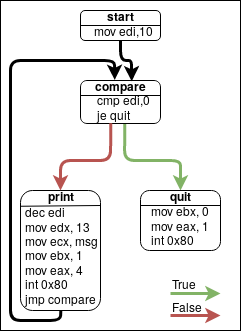
\includegraphics[scale=0.6]{Images/BBGExample.png}
    \caption[The BBG of the "Hello World!" Program.]{The BBG of the "Hello World!" Program. True and false branch conditions are illustrated with green and red arrows respectively.}
    \label{fig:HelloBBG}
\end{figure}
\noindent
\begin{figure}[th]
    \centering
    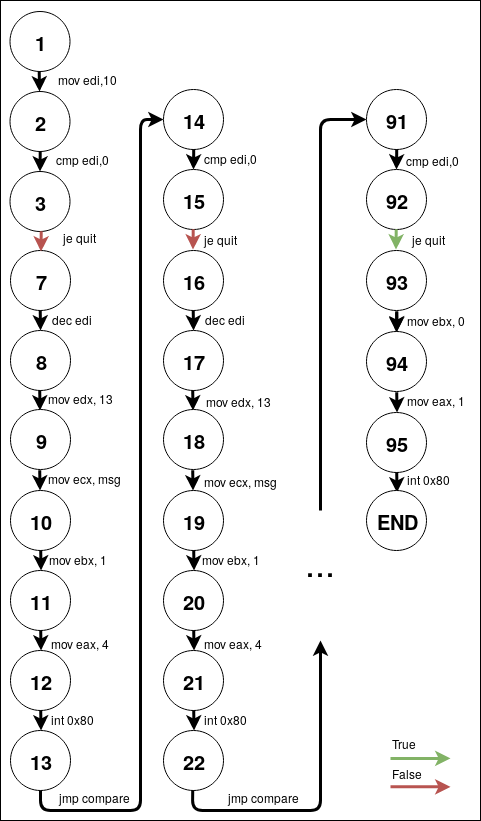
\includegraphics[scale=0.4]{Images/CFA.png}
    \caption[The generalized CFA of the "Hello World!" Program where nodes encompasses all register and memory information.]{The generalized CFA of the "Hello World!" Program where nodes encompasses all register and memory information. True and false branch conditions are illustrated with green and red arrows respectively.}
    \label{fig:HelloCFA}
\end{figure}
\noindent
\\ \\
Assume that the criterion of the nodes of the generalized CFA is based on the complete register and memory content. Then, the generalized CFA of the hello-world program, depicted in Figure \ref{fig:HelloCFA}, only contains one possible path. This is because a node is no longer a group of instructions but rather a set of register values and a set representing memory content, thus accurately representing a concrete state. Consequently, state 2, 14 and 91 are distinct as they differ in the $edi$ value. More specifically, in this example, state 2, 14 and 91 correspond to $edi=10$, $edi=9$ and $edi=0$ respectively. Note, that the conditional jump instruction $je quit$ does not have to correspond to two possible edges as the condition can be fully determined by the state.
%Add assumptions for figure 2.3(CFA of helloworld, i.e abs dom models all reg and mem content  note no socket, random numbers or file reads!)
%Add example depicting a bad abstraction that does not have deterministic state transitions.
%CFA with loop terminates but CFA without loop we don't know if it terminates
\\ \\
A problem with the usage of BBG:s when representing control flow is, for example, when conducting control flow integrity enforcement\cite{CFIEnforcement}. When Control flow integrity enforcement is performed, the auditing software performing this enforcement uses information about what instructions can transfer control flow to which locations. It then audits executing programs to verify that all control flow transfers are performed according to these targets. If, however, a BBG is used, an attacker could enter a basic block from one edge and exit from an edge that shouldn't be feasible in practice when the entry edge was used. For example, if an attacker could manipulate the control flow of the hello world program so that it executed start, check and quit, this would be undetected by the control flow integrity enforcement. This problem is not solved by simply converting the BBG to a CFA representation of the control flow. Rather, one would need to generate and use a sufficiently accurate generalized CFA as this represenation would be able to distinguish between different concrete states at the same location.
%Mention example of control flow integrity(A CFG overapproximates double function calls, thus, using control flow hijacking it is possible to jump somewhere it shouldn't be possible)
% Soundess + completness example in graph + Cascading loss of precision
\begin{figure}[th]
    \centering
    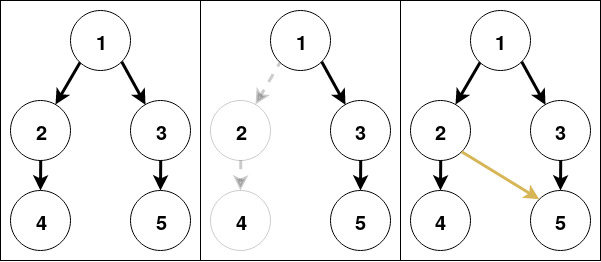
\includegraphics[scale=0.6]{Images/SoundCompleteGraph.png}
    \caption[An example of soundness and completeness in CFG:s.]{An example of soundness and completeness in CFG:s. The leftmost graph is the ideal CFG, the middlemost graph is a complete approximation of the ideal CFG and the rightmost graph is a sound approximation of the ideal CFG. The transparent nodes/arrows denote unidentified parts of the graph and yellow arrows denotes falsely identified edges.}
    \label{fig:SoundCompleteGraph}
\end{figure}
\\ \\
Two desirable properties of CFG:s are soundness and completeness\cite{angr}. Soundness is defined as the extent to which the CFG contains the correct control flow transitions. Thus a CFG is said to be sound if and only if, it contains all the possible control flow transitions. Similarly, completeness of a CFG is the extent to which the CFG only contains possible control flow transitions. Consequently, a CFG is said to be complete if and only if, it only contains possible control flow transfers. 
\\ \\
In Figure \ref{fig:SoundCompleteGraph} the ideal CFG, a complete under-approximation of the ideal CFG and a sound over-approximation of the CFG for some fictional binary program, is presented. The middlemost graph is complete since it contains all edges of the ideal graph. However, during reconstruction of middle most CFG, the edge between node 1 and 2 was missed. Consequently, all nodes after 2 were missed as well. One could imagine that there could be more instructions after node 2 that could only be reached through the edge between node 1 and 2. Thus, missing one edge during the control flow graph reconstruction can lead to a cascading loss of precision. The rightmost graph of Figure \ref{fig:SoundCompleteGraph} is a sound over-approximation of the ideal CFG.
\\ \\
The only problem with the rightmost CFG is that the edge between node 2 and 5 has been added. This might, at first glance, not seem very problematic. However, it can, for example, be a security risk during control flow integrity enforcement. Furthermore, if there are a large amount of falsely identified nodes or edges the reconstruction time and memory usage can be significantly affected. In other words, over-approximation can consume significantly more time and memory resources than under-approximation since it has to explore more nodes and edges\cite{alternating}.
\\ \\
As there are currently no known polynomial time algorithms for creating the optimal CFG of an arbitrary binary, several researchers have resorted to under and/or over-approximation approaches\cite{preciseCFGBoolean}\cite{preciseCFG}\cite{CFGFromPowerPC}\cite{angr}. As purely over-approximating approaches, by definition, does not miss any edges of the ideal CFG, they are sound. Conversely, as under-approximation approaches never include superfluous edges, they are complete. In this thesis we are, however, only interested in the precision of the generated CFG.
\\ \\
The preciseness of a CFG can informally be thought of as the difference in the amount of edges and nodes of the subject CFG and the ideal CFG. Thus, a complete CFG with 10 superflous edges is more precise than a complete CFG with 20 superflous edges. A formal definition of preciseness of a CFG is provided in section \ref{sec:metrics}.
\\ \\
Unresolved control flow transitions primarily stems from the difficulty in resolving indirect jumps. Resolving indirect jumps requires data flow analysis which requires a CFG. However, CFG reconstruction requires resolving indirect jumps. Thus, there is a circular dependency. In the context of static analysis, this circular dependency is referred to as the "chicken and egg" problem\cite{Jakstab}.
%\\ \\
%In this work we do not distinguish between intra and inter-procedural branch instructions. Consequently, we do not use intra-procedural and inter-procedural CFG:s.

%-(Precise Control Flow Reconstruction Using Boolean Logic)-
%"Apart from switch-case statements, compilers generate indirect jumps/calls for function pointers or virtual methods."
%"Indirect control poses a so-called chicken-and-egg problem: In order to reconstruct the control flow graph from binary code, it is necessary to infer invariants that describe those registers which affect the target of an indirect jump/call."
%"the lack of a precise control flow graph often implies a drastic loss in terms of precision for any subsequent verification effort"
%
%Delay slots? 
%"Fortunately most compilers generate indirect jumps only in special cases" (Generic CFG)
%
%"Detecting the basic blocks of a binary program for a RISC-architecture is straightforward"(On the static analysis.. src 'Compilers, principles, techniques and tools')
%
%-(BitBlaze a New Approach...)-
%"Resolving indirect jumps usually requires program analyses that require a CFG"
%"Most normal analyses will first run an indirect jump resolution analysis in order to build a more precise CFG that resolves indirect jumps to a list of possible jump targets."
%VLIW makes things complicated because IP can jump in the middle of an instruction
%Explain why a very precise CFG reconstruction is important(Cascading loss of precision else-way).
%In this work we work with a CFA since these are better than CFG for expansions towards more analysis(since they are context sensitive and thus more expressive)
%CFA has distinct states for same instructions. This is similar to software model checking.

%Maybe mention that the generalized CFA can depict loop unrollment.

%Jakstab: "Call strings, however, are tied to the concept of procedures (which is unreliable in x86 assembly) and assume the existence of a separate call stack. This issue lead to the design of the path sensitive analysis presented in this dissertation."(Comparing jakstab with codesurfer)

\section{Static and Dynamic Analysis}
%https://www.cs.cmu.edu/~aldrich/courses/654-sp08/slides/11-dataflow.pdf "static analysis can find mechanical errors" p7
%Binary Analysis platforms. Microsoft Boogie, Valgrind, LLVM and Mayhem.
%see "static Disassembly and Code Analysis"
%Techniques such as abstract interpretation, constraint solving, and type systems may be used for control-flow analysis.
The goal of static and dynamic analysis techniques are to determine properties and
functions of a program\cite{staticOfInd}. Static analysis is an umbrella term for all methods of program analysis which are conducted by examining a program without subjecting it to any concrete executions. Conversely, dynamic analysis comprises all of the program analysis techniques which are based on concrete executions of the studied program. Furthermore, when the two types of techniques are mixed together, they are sometimes referred to as glass-box testing techniques\cite{DefinitionStaticAnal}.
\\ \\
Binary analysis platforms which leverage Static analysis techniques usually constitute of a hardware-independent representation, a mechanism to translate architecture dependent binaries to this representation as well as several architecture independent analyses that processes the hardware-independent representation\cite{TrABin}. Formally, the intermediate representation is normally represented using abstract interpretation\cite{Jakstab}. Abstract interpretation will be further described in section \ref{sec:AbsInt}.
\subsection{Disassembly in Static Analysis}
A core issue related to the analysis of programs is the undecidable problem of distinguishing code from data\cite{ABinaryRewriting}. As a consequence, static analysis techniques require some sort of techniques which identify what bytes of a binary should be disassembled and then disassembles these bytes. These techniques are referred to as static disassembly techniques. Static disassembly techniques can, in general, be categorized as either being based on either a linear sweep approach or recursive traversal approach\cite{DisassemblyOfExecutable}. It should, however, be noted that none of these two approach are 100\% precise\cite{ABinaryRewriting}. Furthermore, there are also techniques which can not be categorized into these two categories such as, for example, speculative disassembly\cite{preciseCFG}.
\\ \\
Linear sweep approaches starts by disassembling the first byte at the start of a the code section and then simply disassembles one byte after the other until an illegal instruction is encountered\cite{ABinaryRewriting}. This makes linear sweep based disassemblers easy to thwart as an attacker can simply place a jump in front of some malformed instructions. This would make the control flow follow the jump instruction to pass the malformed code but could stop linear sweep disassemblers as they could potentially be unable to disassemble the malformed instructions\cite{ABinaryRewriting}. Some examples of linear disassembly tools are objdump, WinDbg and SoftICE\cite{ReversingSecretsofReverseEngineering}.
\\ \\ 
Recursive traversal approaches starts at the beginning of the code section as lineaer sweep approaches. However, instead of treating branch instructions as fall-through edges, recursive traversal approaches proceed by following each branch instruction encountered in a depth-first or breadth-first manner. Some examples of popular tools that use recursive disassembly are IDA Pro, OllyDbg and PEBrowse Professional\cite{ReversingSecretsofReverseEngineering}.
%See jakstab section 1.2
\subsection{Challenges of Static Analysis}
Apart from the limitations related to disassembly, static analysis also faces other challenges. One such challenge is 
\\ \\
Static analysis can be further complicated when analyzing malware as malware can use techniques that obfuscate the binary representation of a program\cite{StaticDisAndCodeAnal}. For example, malware does not have to comply to calling conventions or use the ABI in according to conventions. Thus, robust techniques are required that can deliver reliable results even when exposed to binries which to not follow conventions. For example, Giovanni Vigna introduced a disassembly technique which can deal with obfuscated binaries by using ..\cite{StaticDisAndCodeAnal}. 
\\ \\
%Challenges
%VLIW -> jumping in the middleo of another instruction,
In this work, both static and dynamic analysis techniques are used to reconstruct a precise CFA from a given binary. Static analysis is used to over-approximate the CFA while dynamic analysis is used to under-approximate targets of unresolved jumps. The over-approximation is conducted using abstract domains which represent an over-approximation of possible variable for various registers and memory locations. Furthermore, directed symbolic execution is combined with a sat-solver to generate program input that executes a specific sequence of instructions that end in an unresolved branch. This input is then fed to the program and an under-approximation is determined for the unresolved branch. A more detailed description of our approach is provided in chapter \ref{chap:methodlogy}.

\subsection{Dynamic Analysis}
%-(Precise Control Flow Reconstruction Using Boolean Logic)-
%Traditional static techniques disassemble a program’s
%binary image statically and build the control flow graph (CFG) from
%the assembly-level representation of the program. They are limited
%in precision because of difficulty in statically resolving indirect
%branches. Dynamic techniques, on the other hand, suffer from poor
%coverage and scalability. Hybrid techniques based on combined
%dynamic and symbolic path exploration can improve code coverage,
%but still suffer from poor coverage and scalability because they rely
%on expensive constraint solving to generate alternative inputs to
%explore different control flow paths.

\section{Abstract Interpretation}\label{sec:AbsInt}
%See summary of https://www.youtube.com/watch?v=EF_6QaQ_M-s&t=20s
Abstract interpretation is a technique where concrete objects are represented as abstract objects. In general, there is a monotonic function, denoted by $\alpha$, converting a concrete element into its corresponding abstract representation. This function is usually referred to as the abstraction or representation function. Conversely, there is a monotonic function, denoted by $\gamma$, converting an abstract object into its corresponding concrete object. This function is referred to as the concretization function
\\ \\%Is this rice's theorem? 
The reason for not carrying out analysis directly using concrete semantics is that it is not possible to create a program which is able to represent and compute all possible executions of any program in all its possible execution environments\parencite{FRPatrick}. Consequently, all non-trivial questions about the concrete semantics of a program are undecidable. However, if one uses abstraction to only include properties which are of interest to the analysis, it can be possible to analyze the selected properties in finite time. Thus, by abstracting a program to an abstract interpretation, it is possible to analyze the relevant properties in less than infinite time.
\\ \\
To be able to understand abstract interpretation, one first need to understand partially ordered sets\parencite{EoMPoset}, correspondence\parencite{EoMCorrespondence} and Galois connections\cite{galoisConnections}. A partially ordered set(poset) consists of a set and a binary relation such that the binary relation, given two elements, indicate which of the elements should precede the other or that neither of them precedes the other. Additionally, the binary relation must be reflexive, anti-symmetric and transitive. The difference between partially and totally ordered sets is that the former allows elements in the set to be incomparable while the latter requires every pair of elements, belonging to the set, to be comparable.
\\ \\
A correspondence is a generalization of a binary relation which operators on two sets or mathematical structures of the same type. A correspondence between two sets A and B is any subset of $A \times B$. A Galois connection is a correspondence between two partially ordered sets. There are two types of galois connections: monotone and antitone. This thesis uses monotone galois connections. Consequently, when a galois connection is mentioned, it reefers to a monotone galois connection.
\begin{definition} \textbf{Galois Connection}\\
Let $(A, \sqsupseteq_A)$ and $(B, \sqsupseteq_B)$ be two partially ordered sets. Furthermore, let F and G be monotone functions such that  $F : A \rightarrow B$ and $G : B \rightarrow A$. Then, ${(A, \sqsupseteq_A)}$, (B, $\sqsupseteq_B$), $F$ and $G$ form a Galois connection  if for all $a \in A$ and $b \in B$:
\makebox[\linewidth]{$F(a) \sqsupseteq_B b$ if and only if $a \sqsupseteq_A G(b)$}
\end{definition}
\noindent
In abstract interpretation, a Galois connection is established between a concrete and an abstract domain. The abstraction function $\alpha$ and the concretization function $\gamma$ correspond to the functions F and G in the definition above. Furthermore, the two posets in the definition corresponds to the abstract and concrete domain. More specifically, in abstract interpretation, the posets are typically bounded lattices.
\\ \\%https://en.wikipedia.org/wiki/Lattice_(order)
A lattice is a poset where every pair of elements have a unique least upper bound and a unique greatest lower bound. The least upper bound is also known as the supremum or join. Similarly, the greatest lower bound is also known as the infimum or meet. Furthermore, if a poset only satisfiy the requirement that each pair of elements have a unique least upper bound it is a join-semilattice. Similarly, if a poset only satisfiy the requirement that each pair of elements have a unique greates lower bound it is a join-semilattice. Thus, a lattice could also be defined as a poset which is both a join-semilattice and a meet-semilattice.
\\ \\
A bounded lattice is a lattice which has a top element $\top$ and a bottom element $\bot$ such that, for all lattice elements x, $\bot \leq x \leq \top$. Equivalently, a lattice is a bounded lattice if and only if every finite set of elements has a join and a meet. 

%Galois connections between concrete and abstract semantics, widenings and narrowings

%Complete lattice?
%Abstract Domain

%Ascending chain condition

%Abstract semantics are a superset of the concrete semantics (https://www.di.ens.fr/~cousot/AI/IntroAbsInt.html#Cousot81-1)

%We say that an abstraction is sound (or correct) if the abstract semantics covers all possible cases of the concrete semantics. All formal methods are required to use sound abstractions: if a potential error is not signaled that it should be definitely impossible. Contrary to testing/debugging formal methods provide full coverage.(https://www.di.ens.fr/~cousot/AI/IntroAbsInt.html#Cousot81-1)

%To be a partial order, a binary relation must be reflexive (each element is comparable to itself), antisymmetric (no two different elements precede each other), and transitive (the start of a chain of precedence relations must precede the end of the chain). 

%"Intervals are better than exact sets because with exact sets algorithms used can be guaranted to finish in finite time."(powerpc?) 
%Rice's theorem

%"If the number of assumptions about the code is to be minimized, it is necessary to use an abstract domain for the analysis that is able to precisely represent target addresses." (jakstab)

% The concrete semantics of a program is an "infinite" mathematical object which is not computable: it is not possible to write a program able to represent and to compute all possible executions of any program in all its possible execution environments. Hence, all non trivial questions about the concrete semantics of a program are undecidable: it is not possible to write a program able to answer any question about the possible executions of any program (since the concrete semantics of this program would have to be computable). https://www.di.ens.fr/~cousot/AI/IntroAbsInt.html

%The join and meet of a subset S are respectively the supremum (least upper bound) of S, denoted ⋁S, and infimum
%A partially ordered set that is both a join-semilattice and a meet-semilattice is a lattice.
%https://en.wikipedia.org/wiki/Join_and_meet

\section{Under-Approximation Approaches}
%Add small probability of reaching if (x=564) when doing random input generation.
An approach to under-approximate the control flow of a binary is to execute the binary with some carefully generated input and then add the execution trace to the control flow graph. To craft this input, it is possible to use fuzzing techniques or symbolic execution.
\\ \\
Fuzzing techniques are in general categorized as black-box, gray-box or white-box techniques\cite{fuzzingSurvey}. Black-box techniques are techniques which treats the Program Under Test(PUT) as a black box. Thus, black-box techniques only observes the input and output of the PUT. Conversely, white-box techniques are techniques which exploit knowledge of the internals of the PUT. Furthermore, Gray-box techniques are techniques which can not be categorized as purely white or black-box as they uses a mixture of the two techniques. As black box fuzzing typically exhibits low coverage, black-box techniques are typically not of interest in the context of CFG reconstruction\cite{fuzzingSurvey}.
\\ \\
A popular gray-box technique is mutation-based fuzzing. Mutation based fuzzers takes an initial seed which is an initial well-formed input. Thereafter, the seed is given to the PUT and some information from the execution is obtained. This information is then used to create new seeds by mutating existing ones. Common mutation techniques are bit-flipping, arithmetic mutation, block-based mutation and semantic mutation\cite{fuzzingSurvey}.
\\ \\ 
White-box techniques are usually some sort of guided fuzzing, PUT mutation or Dynamic Symbolic Execution (DSE)\cite{fuzzingSurvey}. Guided fuzzing encompasses all techniques which leverage static or dynamic program analysis techniques for enhancing the effectiveness of the fuzzing process. PUT mutation includes techniques which modify the PUT in a way that benefits the generated input seeds. For example, PUT mutation can be used to remove a checksum check in a PUT, to ensure that all input pass the check\cite{fuzzingSurvey}.
\\ \\
During DSE, which is also known as concolic execution, the program is initially executed with an initial input. The input is then given to the PUT in what is denoted as a concrete execution. During the concrete execution, symbolic expressions are recorded for the passed branches. Thereafter, an smt solver can be given a variation of the obtained constraints to create a set of inputs that would take a specific path in the binary. This technique is has the advantage of being more likely to generate inputs that improve coverage than random inputs. On the other hand, a disadvantage of using whitebox techniques is that they are often slower than gray or black-box techniques. 
\\ \\
Constraint-based fuzzing techniques like DSE focus on solving constraints to create inputs that take different paths in the PUT. Consequently, this is a more attractive technique than mutation based fuzzing when one wants to reconstruct the control flow of a PUT.

%remove the things below
Therefore, this project focused on developing a DSE with a score-based algorithm similarly to the algorithm used by Godefroid et al\cite{automatedFuzzing}. This algorithm used a score-based evaluation to ensure that the generated input values result in the usage of as many new branches as possible. Consequently, maximizing the amount of new CFG edges with respect to the number of calls to the expensive SMT solver\cite{automatedFuzzing}. Consequently, the path explosion problem is mitigated, favoring scalability.
\\ \\
In this thesis, we conduct Directed Symbolic Execution(DSE) not to be confused with Dynamic Symbolic Execution.

%In this project we take inspiration from fuzzing techniques to address the problem of under-approximating CFGs.
%"What you fuzz is what you chip" https://queue.acm.org/detail.cfm?id=2094081

%Example with if x = 2 is very unlnikely to be caught by black box
%"This problem motivates the use of seed-based input generation as well as white-box input generation" (fuzzing Survey from 2019)
%Explain why white-box fuzz-testing

%https://homepages.dcc.ufmg.br/~fernando/classes/dcc888/ementa/slides/WorkList.pdf Worklist algo
%https://www.cs.cmu.edu/afs/cs/academic/class/15745-s03/public/lectures/L4_handouts.pdf
\section{Dataflow Analysis}
Dataflow analysis is the problem of, for each program location, assigning a lattice element which over-approximates the possible concrete states at that program location\cite{cpaAlgo}. Usually dataflow analysis uses the program's BBG to determine to which parts of the program, values of variables might propagate. The most precise over-approximation can be determined by determining the least fixpoint. This can be done by applying the transfer relation to abstract states and join the result with previous result at the corresponding program location. To determine whether the fixpoint has been reached or not, it is common to use a worklist which stores dataflow facts\cite{cpaAlgo}.
\\ \\
Techniques for dataflow analysis can be categorized into two categories; forward flow and backward flow analysis. In forward flow analysis, each exit node of a basic block is expressed as a function of the entry node of the basic block. Conversely, in backward flow analysis, entry nodes are expressed as functions exit node of the corresponding basic blocks. This funciton is referred to as the transfer function. The semantics of the transition function is defined by the semantics of the instructions inside the basic blocks. Forward analysis typically requires an initial entry state to be defined. This entry state is used as the starting point o the propagation of dataflow information and can, for example, contain the fact that no variables have any known values. Similarly, backward flow analysis requires an initial exit state to be known. Examples of forward and backward flow analysis techniques are reaching definitions and liveness analysis respectively.
\\ \\
It is possible to conduct dataflow analysis techniques on a different granularity than basic blocks. For example, they can be conducted on the instruction level, using a relation between the entry node and exit node of each instruction. This is normally referred to as local analysis\cite{carneigeDataFlow}. However, it is more common to work at the basic block level and then use local analysis inside basic blocks when instruction-level dataflow information is desired\cite{carneigeDataFlow}.
%http://web.cs.iastate.edu/~weile/cs641/5.DataFlowAnalysis.pdf
\begin{figure}[t]
    \centering
\begin{lstlisting}[escapeinside={(*}{*)},style=algorithm]
in[$B_s$] := $X_0$
for each basic block $B$
    out[$B$] := $\top$
    
$worklist$ = {$B$: for all basic blocks $B$}
while($worklist \neq \emptyset$)
    $B$ := remove($worklist$)
    in[$B$] := $\sqcap$ {out[$B^{'}$]: $B^{'}$ $\in$ pred($B$)}
    
    if out[$B$] $\neq$  $F_B($in[$B$]$)$
        $worklist$ := $worklist$ $\cup$ succ($B$)
        out[$B$] := $F_B($in[$B$]$)$
\end{lstlisting}
\caption[Example of a forward flow analysis worklist algorithm.]{Example of a forward flow analysis worklist algorithm.}
    \label{fig:WorklistAlgo}
\end{figure}
\noindent
\\ \\
An example of a worklist algorithm for a forward flow analysis is provided in figure \ref{fig:WorklistAlgo}. This algorithm assumes that a BBG is available to determine the predecessors pred(B) and successors succ(B) of a basic block B. Furthermore, the information of the entry and exit of a basic block B is denoted by in[B] and out[B] respectively. Initially, the  input information of the starting block $B_s$, is set to a specific pre-defined value $X_0$. For each basic block, the exit information is then set to top, meaning that no information is known. The worklist is then initially filled with all basic blocks of the BBG and the while-loop is entered.
\\ \\
In the while loop, a random basic block B is removed from the worklist. The entry information of this block is then recalculated depending on the information of its predecessors. Then, the algorithm checks if the new output of $B$, obtained by applying the transfer function $F_B$ to the input information of $B$, is different from the previous output information of B. If this is the case, the output information of B is updated with the new generated information and all successors of B are re-added to the worklist as their input information is dependent on the output information of B.
\\ \\
As dataflow requires the BBG whose reconstruction is dependent of dataflow facts, it is not trivial how one would reconstruct one without the other. However, Kinder\cite{Jakstab} devised an algorithm that can perform CFA reconstruction and deductions of dataflow facts simultaneously. In this thesis, this algorithm is used for the over-approximation part of the alternating approach presented in chapter \ref{chap:methodlogy}.
\\ \\ 
Dataflow analysis can for example be used for code optimization by avoiding redundant or superflous computations. Furthermore, it can also be used for code validation through invariant generation\cite{BordeauxSoftwareVerification}.


%Worklist algorithm: https://en.wikipedia.org/wiki/Reaching_definition


%\section{Application Binary Interface}
%An Application binary interface(ABI) defines the rules of communication between a binary and the underlying operating system.

%\section{ELF structure}

\section{Over-Approximation with Jakstab}
Jakstab\cite{Jakstab} is an abstract interpretation based static analysis framework which combines control flow and data flow analysis to resolve the chicken and egg problem of control flow reconstruction. It uses on-demand disassembly and an intermediate language to over-approximate the CFA of a binary.
\\ \\
To abstract the details of assembly language while still capturing its relevant branching behaviour, Jakstab uses and intermediate language(IL). Furthermore, the author of the platform defines a set of statements denoted by \textbf{Stmt}. Assume that $e_1,e_2 \in Exp$ where $Exp$ is the set of possible expressions. Then, the set \textbf{Stmt} consists of memory assignments $m[e_1] := e_2$,conditional indirect jumps $if\:e1\:jmp\:e2$, assume statements $assume\:e1$ and a halt statement $halt$.
\\ \\
The only data type of the IL is integers. Consequently, booleans are represented by 0 for false and 1 for true. Furthermore, the finite set of program locations is denoted by $L \subseteq N$.This set contains all addresses of the program. A program is denoted as $<\ell_0,P>$ where $\ell$ is a starting location and $P$ is a finite mapping from program locations to statements and successors, More formally, $P$ is defined as $P:: L \rightarrow (Stmt \times L)$. In this thesis, the statement stmt at location $\ell \in L$ with successor $\ell^{'}$ is denoted by $[stmt]^{\ell}_{\ell^{'}}$ 

Unresolvable jumps are usually referred to as tops ($\top$) as they can contain any lattice element.

\section{Abstract Domains}
In this section the abstract domains used for the over-approximation are briefly and informally introduced. All of the abstract domains have a corresponding formal definition in Kinder's dissertation\cite{Jakstab}. First, the location analysis domain is briefly described in section \ref{sec:absDomLoc}. Thereafter, the constant propagation domain is explained in section \ref{sec:absDomCon}. Finally, the strided interval analysis is detailed in section \ref{sec:absDomInt}. These sections will contain assembly examples to illustrate when they are useful. For these and other assembly code examples, each line of code will be paired with a comment to help readers unfamiliar with x86 assembly.

\subsection{Location Analysis}\label{sec:absDomLoc}
The location analysis domain allows to omit location information from other abstract domains. It contains a label of an intermediate level instruction, which is an address to a concrete instruction and an index as each concrete instruction can correspond to multiple intermediate level instructions. The location Analysis is never used on its own, instead it is always combined with another abstract domain.

\subsection{Constant Propagation}\label{sec:absDomCon}
The constant propagation domain consists of constant propagation and constant folding. Constant propagation is when constants are propagated through instructions so that operand registers can be substituted with concrete values. Furthermore, constant folding significates that constant expressions are calculated and substituted by the result of their evaluation.
\\ \\
For example, consider the synthetic program \it{cjmp.asm} depicted in Figure\ref{fig:cjmp.asm}. The text section is the section containing the instructions of a binary. Its start is declared line 1. Then, line 2 declares the \it{\_start} label to be global, making it possible for the linker to know where the binary should start. The binary starts at line 5 by moving the constant value 0 into the register eax. Thereafter, through line 6 to 10, a series of registers operations are performed. These operations results in the the values 0 and 22 to be stored in the \it{eax} and \it{edi} register respectively. The \it{cmp} instruction at line 11 is then executed to set the flags according to the comparison between eax and 0. Since eax is 0, the zero flag \it{ZF} is set to one. Consequently, the instruction on line 12, which performs a jump to \it{exit} if \it{ZF} is set, jumps to \it{exit} and the program terminates. 

\begin{figure}[!ht]
    \centering
\begin{tcolorbox}
\begin{minted}[xleftmargin=5pt,linenos,fontsize=\footnotesize]{nasm}
SECTION .text
global _start

_start:
        mov eax, 0      ; eax = 0
        add eax, 20     ; eax = eax + 20
        mov edi, 12     ; edi = 12
        sub eax, 30     ; eax = eax - 30
        add edi, 10     : edi = edi + 10
        add eax, 10     ; eax = eax + 10
        cmp eax, 0      ; Compare eax with 0
        je exit         ; if ZF=1 jump to <exit>
unreachable:            
        jmp unreachable ; Jump infinitely
exit:
        mov ebx, 0      ; Set exit code to 0
        mov eax, 1      ; Set eax to sys_exit
        int 0x80        ; Syscall
\end{minted}
\end{tcolorbox}
\caption[]{cjmp.asm - an example containing a conditional jump which can be resolved without false positives using the constant propagation domain.}
    \label{fig:cjmp.asm}
\end{figure}
\noindent
Evaluation using the constant propagation domain starts with an empty state. The first instruction is then parsed into an instruction \it{eax = 0} and the value of 0 is stored in the register eax. Then, the next instruction is parsed resulting in the instruction \it{eax = eax + 30}. At this point, the value \it{eax = 0} is propagated to this instruction, turning it into the instruction \it{eax = 0 + 20} which is simplified to \it{eax = 20} and stored in the new state. The next instruction, at line 7, is parsed and the state is updated to hold the values \it{\{eax=20,edi=12\}}. 
\\ \\
The next instruction \it{eax = eax - 30} is loaded, \it{eax} is substituted with 20 and constant folding is performed to obtain the state \it{\{eax=-10,edi=12\}}. Thereafter, the same procedure repeats for the last two instructions \it{edi = edi + 10} and \it{eax = eax + 20} resulting in the state \it{\{eax=0,edi=22\}}. Now, the constant value of \it{eax} can be propagated to the succeeding compare instruction substituting eax in the expression and resulting in the instruction \it{cmp 0,0}. Consequently, the \it{ZF} flag can be determined to be one and the jump instruction at line 12 can be determined to only have the successor at line 16, eliminating a false positive edge in the CFA to the unreachable jump instruction.
\\ \\
While constant propagation has the benefit of being able to scale well to larger programs\cite{alternating}, it has the disadvantage of not being able to resolve successors of return instructions. The reason is that constant propagation does not capture the effect of the call function and does thus not know what address is at the top of the stack when the return instruction is later executed.

\subsection{Strided Intervals}\label{sec:absDomInt}
The elements of the strided interval domain consists of tuples with three elements. These three elements are integers for a minimum, maximum and a stride value. More formally, a strided interval is defined as: 
\begin{definition}\textbf{Strided Interval}\\
A strided interval is an interval $s[l,u] = \{l + s * n\;|\;l \leq l + s * n \leq u, n \in N \}$ where $s,l,u \in N$ and $N$ is the set of natural numbers including the zero element.
\end{definition}
\noindent The stride of a strided interval can be thought of as the difference between two adjacent elements of the interval. For example, the interval $2[4,8]$ is equivalent to the set $\{4,6,8\}$ since it contains the lower bound 4 and values separated by a stride of 2 up to the upper bound 8. As a consequence, conventional intervals can be represented as strided intervals where the stride is equal to 1. Furthmore, a stride of 0 significates a singleton set containing only the lower bound of the interval, for example, $0[2,2] = 2$
\begin{figure}[ht]
    \centering
\begin{tcolorbox}
\begin{minted}[xleftmargin=5pt,linenos,fontsize=\footnotesize]{nasm}
SECTION .bss
buf      resb 4                 ; Reserve 4 bytes of
                                ; memory
SECTION .text
global _start

increment:
        add ebx, 1              ; ebx = ebx + 1
        jmp continue            ; jump to <continue>
_start:
        mov  edx, 4             ; length of buffer
        mov  ecx, buf           ; pointer to buffer
        mov  ebx, 0             ; stdin
        mov  eax, 3             ; sys_read
        int  0x80               ; perform syscall

        mov eax, dword [buf]    ; eax = T
        mov ebx,0               ; ebx = 0
        cmp eax,1               ; compare eax with 1
        je increment            ; if eax = 1 jump
                                ; to <increment>
continue:
        add ebx, exit           ; ebx = ebx + <exit>
        jmp ebx                 ; jump to ebx
exit:
        nop                     ; No operation (1 byte)
        mov ebx, 0              ; Set exit code to 0
        mov eax, 1              ; sys_exit
        int 0x80                ; Syscall
\end{minted}
\end{tcolorbox}
\caption{branch.asm - an example of when strided intervals can be more useful than constant propagation.}
    \label{fig:branch.asm}
\end{figure}
\noindent
Strided intervals are useful to represent program locations where a register or memory location can contain more than one value. We will illustrate this through an example. Consider the assembly code of \it{branch.asm} depicted in Figure \ref{fig:branch.asm}. In addition to the text section, we instruct the basic service set(bss) section to reserve one byte for our program at line 2. 
\\ \\
When executed, the program begins at the \it{start} label and starts by setting up the registers to perform a system call using \it{sys\_read}. At line 15, the CPU is instructed to perform the system call to read one byte from standard input into the buffer buf which is located in the bss section. This is done by performing a context-switch where the CPU is put in kernel mode where it has additional privileges and can perform the read into the buffer. The CPU then performs the read followed by a transition into user mode and a context switch resuming the execution of the program at the instruction after the syscall instruction.
\\ \\ 
At line 17 the content of \it{buf}, which contains the first 32 bits of the user's input, are copied into the 32-bit register \it{eax}. Thereafter, the \it{ebx} register is initialized 0, as it will be used as a counter. Then, \it{eax} is compared with 1 to determine if control should be transfered to the \it{increment} label or directly to the \label{continue}- In the first case, the CPU executes line 8 to increase \it{ebx} by 1 and then jumps to line 23. At line 23 the offset of the \it{exit} label is added to the \it{ebx} register. Afterwards, a jump to the content of \it{ebx} is performed. At this point, \it{ebx} is either equal to \it{exit} or \it{exit + 1}. Note, however, that the instruction located at \it{exit} is a \it{nop} instruction of size 1 byte. Consequently, the CPU will execute either the \it{nop} instruction and continue from line 27 or continue from line 27 directly. Thus, the semantics of the program are independent of the user input. 
\\ \\
At the start of execution the interval analysis starts with a state only containing a strided interval with a stride of 0 for the stack pointer. After exxecuting the syscall, each of the four registers used to pass parameters to the syscall, are represented by intervals of a stride of 0. Then, the \it{mov} instruction at line 17 is executed to load the content of the buffer into the \it{eax} register. However, as it is impossible to determine what user input is entered without actually executing the program, it is not possible to know what \it{buf} will contain after the syscall and thus not what will be loaded into the \it{eax} register at line 17. Consequently, the strided interval for eax will be removed from the state, i.e \it{\{eax=0[3,3], ebx=0[0,0], ecx=0[buf,buf], edx=0[4,4]\}} becomes \it{\{ebx=0[0,0], ecx=0[buf,buf], edx=0[4,4]\}}.
\\ \\
After loading the content of buf into eax, the ebx register is set to 0 and then the eax register is compared with 1. However, as there is currently no knowledge of eax in the state, it has to be assumed that all different flag values are possible after this statement. Consequently, when the \it{je increment} statement is reached, it has to be assumed that execution can continue on either line 8 or 23. Consequently, the state is split into one state where \it{ZF=1} and the execution continues at line 8 as well as one where \it{ZF=0} and the execution continues at line 23. The analysis which continued on line 8 will increase the value of \it{ebx} by 1 by changing the strided interval \it{0[0,0]} to \it{0[1,1]}. Then, the jump instruction is taken to line 23. Now there are two states which can be merged at this location, resulting in a state containing a wider strided interval \it{ebx=1[0,1]]}. The \it{exit} label is then added to the interval of \it{ebx} and the indirect jump to the content of \it{ebx} is performed. Since, a strided interval can model the two possible values of ebx, it can be determined that \it{jmp ebx} results in a jump to either \it{nop} or \it{mov ebx, 1} at line 26 or 27 respectively. The state is then propagated through the last instructions to the system call to \it{sys\_exit}.
\\ \\
If, constant propagation would have been used to analyse the binary, the two states at line 23 would not have been possible to merge as they would have two different values for \it{ebx} and constant propagation only allows a state to hold at most 1 value per register and memory location.

\section{Fundamentals of Symbolic Execution}

\chapter{Methodology}\label{chap:methodlogy}
%The choice of method is justified.
%Relevant methods are clearly described and supported by references.
%The methods are used correctly, the technical content is at an appropriate level.

%Explain Limited depth first search in DSE.java of jakstab

%Jakstab: Pesimisitc vs optimistic vs semi-optimistic. Increase coverage?

%Strong vs weak updates? 
Reconstructing the CFA of an arbitrary binary is generally considered to be hard\cite{Jakstab}. In this section, our approach of alternating over/under approximation is presented. %[Describe outline]

\section{Assumptions and Target Binaries}
%---Jakstab assumptions---
% Binaries follow the call conventions and do not contain tail recursion (Double check?)
% No overlapping instructions(Double check?)
%---Manticore assuumptions---
%
%
%---Other limitations---
% No multithreaded binaries as the state space is to large(the order of what thread executes what instructions)
%
%
As the final CFG won't be sound or complete, it won't be of use for binary analysis which requires these properties. For example, it can not be applied to formal verification of binaries as this field requires sound over-approximations. Instead, it is of more use when the goal is to recreate a precise CFG at the cost of the soundness and completness properties. For example, more precise CFGs at the cost of soundness are useful in fields such as reverse engineering as reverse engineers' main desire often is a close to the ideal CFG.
\\ \\
Since there are no restrictions on the target binaries except for general assumptions that are required for constant propagation and the white-box fuzzing, the approach will target all types of binaries that satisfy these assumptions. The first assumption is that the code is not self-modifying, as this would make it close to impossible to over-approximate the targets of indirect branches through static analysis. Another assumption is that the stack can not be modified through pointer dereferences or buffer overflows since this could enable arbitrary control flow graphs. Consequently, as malware often use polymorphism and does not always conform to conventions, there can be no guarantees that the CFG can be recovered from arbitrary malware binaries. Rather, the algorithm would be more interesting for studying well-behaved binaries such as drivers. This can, for example, be useful for corporations who wish to verify that the CFG of the shipped binary is the same as the CFG of the source code.

\begin{itemize}
    \item The global memory region, the stack, and the heap are assumed to not overlap.
    %\item The stack and allocated heap regions are disjoint(same as above..)
    %\item The stack pointer is initialized to a value of 0%??
    \item No pointers escape their allocated memory bounds(I.e no buffer overflows)
    \item Values of arbitrary bit length can be stored at a single store address and no memory locations overlap
\end{itemize}
%CPA framework: https://link.springer.com/content/pdf/10.1007%2F978-3-540-73368-3_51.pdf
%"he intuition of the approach presented here is that the edge relation grows during the fixed point iteration until a simultaneous least fixed point of both data and control flow is reached." -Jakstab

\section{Modifications to the CPA Algorithm}
The CPA algorithm was modified to be able to use the answers provided by the DSE. The Jakstab tool, which is used to over-approximate the control flow, builds upon the Configurable Program Analysis(CPA) framework. The first version of the framework was presented by Beyer et al\cite{cpaAlgo} and contributed with the possibility to combine model checking with program analysis. Later on, Beyer et al extended their algorithm to also include dynamic precision adjustment and referred to the new version of the algorithm as the CPA+ algorithm\cite{cpaPlusAlgo}.
\\ \\
The CPA+ algorithm, presented in Figure \ref{fig:CPAOrig}, is a variant of a standard worklist algorithm. The algorithm is parameterized by a configurable program analysis $\mathcal{D} = (D,\Pi,\rightsquigarrow,$merge$,$stop$,$prec$)$ which consists of an abstract domain $D$, a precision domain $\Pi$, a transfer function $\rightsquigarrow$, a merge operator merge, a stop operator stop and a precision operator prec. These components influence the cost and precision of a program analysis.
%Describe what each component is used for
%Describe the algorithm 
\\ \\
Both the CPA and CPA+ algorithm required a CFA to propagate data flow facts. The contribution by Kinder\cite{Jakstab} was that the CFA would be rebuilt simultaneously to the propagation of the data flow facts. Thus removing the requirement to have a CFA for data flow analysis and potentially providing a solution to the circular dependency between data flow analysis and CFA reconstruction.
\\ \\ 
The modified CPA+ algorithm used in the Jakstab algorithm, created by Kinder, is presented in Figure \ref{fig:CPAJakstab}. The main difference between the Jakstabs version of the CPA+ algorithm and the original CPA+ algorithm is that Jakstab integrates the resolve operator as a call to a transformer factory which provides CFA edges. Thus, the CFA is no longer required as input to the algorithm.
%Some key differences are that reached takes an argument. Diff in out of algo. Uses transformers. More "foreach"

%fix pow ticks (a^{'})
%Change rightarrow to rightsquigarrow
\begin{figure}[thb]
    \centering
\begin{lstlisting}[style=algorithm]
Input: A CPA with dynamic precision adjustment 
    $\mathcal{D}:=(D,\Pi,\rightarrow,$merge$,$stop$,$prec$)$, an initial abstract state $a_0 \in A$ with 
    precision $\pi_0 \in \Pi$ and a CFA as a set of edges G.
Output: A set of reachable abstract states.
$worklist := \{(a_0,\pi_0)\}$
$reached := \{(a_0,\pi_0)\}$
while $worklist \neq \emptyset$
    pop $(a,\pi)$ from $worklist$
    $(\hat{a},\hat{\pi}) := $prec$(a,\pi,reached)$
    foreach $a^{'}$ with $\exists g \in G$. $\hat{a} \xrightarrow{g} (a^{'},\hat{\pi})$
        //Attempt to merge with existing abstract states
        foreach $(a^{''},\pi^{''}) \in reached$
            $a_{new} :=$ merge$(a^{'},a^{''},\hat{\pi})$
            if $a_{new} \neq a^{''}$
                $worklist := (worklist \cup {(a_{new},\hat{\pi})}) \setminus \{(a^{''},\pi^{''})\}$
                $reached := (reached \cup {(a_{new},\hat{\pi})}) \setminus \{(a^{''},\pi^{''})\}$
        //Add new abstract state
        if $\neg$ stop$(a^{'},\{a|(a,\cdot) \in reached \}, \hat{\pi})$
            $worklist := worklist \cup {(a^{'},\hat{\pi})}$
            $reached := reached \cup {(a^{'},\hat{\pi})}$
return $\{ a|(a,\cdot) \in reached \}$
\end{lstlisting}
\caption[The original CPA Algorithm.]{The Original CPA Algorithm.}
    \label{fig:CPAOrig}
\end{figure}


\begin{figure}[thb]
    \centering
\begin{lstlisting}[style=algorithm]
Input: A CPA $\mathcal{D}:=(D,\Pi,\rightarrow,$merge$,$stop$,$prec$)$, an initial abstract state $a_0 \in A$ 
with precision $\pi_0 \in \Pi$ and a map P from locations to statements.
Output: A CFA of P and the set of reachable states.
$worklist := \{(a_0,\pi_0)\}$
$reached(a_0(pc)) := \{(a_0,\pi_0)\}$
$G := \{\}$
while $worklist \neq \emptyset$
    pop $(a,\pi)$ from $worklist$
    $(\hat{a},\hat{\pi}) := $prec$(a,\pi,reached)$
    foreach $g \in $ getTransformers($\hat{a}$,$P$)
        foreach $a^{'}$ with $\hat{a} \xrightarrow{g} (a^{'},\hat{\pi})$
            $G := G \cup g$
            //Attempt to merge with existing abstract states
            foreach $(a^{''},\pi^{''}) \in reached$
                $a_{new} :=$ merge$(a^{'},a^{''},\hat{\pi})$
                if $a_{new} \neq a^{''}$
                    $worklist := (worklist \cup {(a_{new},\hat{\pi})}) \setminus \{(a^{''},\pi^{''})\}$
                    $reached := (reached \cup {(a_{new},\hat{\pi})}) \setminus \{(a^{''},\pi^{''})\}$
            //Add new abstract state
            if $\neg$stop$(a^{'},\{a|(a,\cdot) \in reached \}, \hat{\pi})$
                $worklist := worklist \cup {(a^{'},\hat{\pi})}$
                $reached := reached \cup {(a^{'},\hat{\pi})}$
return $G,\{ a|(a,\cdot) \in reached \}$
\end{lstlisting}
\caption[The CPA Algorithm of Jakstab.]{The CPA Algorithm of Jakstab.}
    \label{fig:CPAJakstab}
\end{figure}

\begin{figure}[thb]
    \centering
\begin{lstlisting}[style=algorithm]
Input: A CPA $\mathcal{D}:=(D,\Pi,\rightarrow,$merge$,$stop$,$prec$)$, an initial abstract state
$a_0 \in A$ with precision $\pi_0 \in \Pi$ and a map P from locations to statements.
Output: A CFA of P and the set of reachable states.
$worklist := \{(a_0,\pi_0)\}$
$reached(a_0(pc)) := \{(a_0,\pi_0)\}$
$G := \{\}$
$unresolved := \{\}$
$DSEEdges := \{\}$
$fixpoint := false$
while $worklist \neq \emptyset$ 
    pop $(a,\pi)$ from $worklist$
    $(\hat{a},\hat{\pi}) :=$ prec$(a,\pi,reached)$
    $DSET := \{(l_1,\cdot,\cdot)|(l_1,\cdot,\cdot)\in DSEEdges \cap l_1 = L(\hat{a})\}$
    $transformers :=$ getTransformers$(\hat{a}$,$P) \cup DSET$
    if $transformers = \emptyset$
        $unresolved := unresolved\; \cup\; (\hat{a},\hat{\pi})$
    foreach $g \in $  $transformers$ 
        foreach $a^{'}$ with $\hat{a} \xrightarrow{g} (a^{'},\hat{\pi})$
            $G := G \cup g$
            //Attempt to merge with existing abstract states
            foreach $(a^{''},\pi^{''}) \in reached$
                $a_{new} :=$ merge$(a^{'},a^{''},\hat{\pi})$
                if $a_{new} \neq a^{''}$
                    $worklist := (worklist \cup {(a_{new},\hat{\pi})}) \setminus \{(a^{''},\pi^{''})\}$
                    $reached := (reached \cup {(a_{new},\hat{\pi})}) \setminus \{(a^{''},\pi^{''})\}$
            //Add new abstract state
            if $\neg$stop$(a^{'},\{a|(a,\cdot) \in reached \}, \hat{\pi})$
                $worklist := worklist \cup {(a^{'},\hat{\pi})}$
                $reached := reached \cup {(a^{'},\hat{\pi})}$
    if $worklist = \emptyset \wedge fixpoint = false$
        $paths :=$ getPaths$(G,unresolved)$
        $G_{old} := G$
        $DSEEdges :=$ DSE$(paths)$
        for $(a,\pi) \in states$ such that $(L(a),\cdot,\cdot)\in DSEEdges$
            $worklist := worklist \cup (a,\pi)$
        $unresolved := \{\}$
        $fixpoint := (G_{old} = G \cup DSEEdges)$
            
return $G,\{ a|(a,\cdot) \in reached \}$
\end{lstlisting}
\caption[Modified version of the CPA Algorithm to include DSE input.]{Modified version of the CPA Algorithm to include DSE input.}
    \label{fig:CPAFinal}
\end{figure}

\clearpage

%Can handle truetops when checking if graph is != previous graph(True top won't be resent forever)

\begin{figure}[thb]
    \centering
\begin{lstlisting}[style=algorithm]
Input: A CPA $\mathcal{D}:=(D,\Pi,\rightarrow,$merge$,$stop$,$prec$)$, an initial abstract state
$a_0 \in A$ with precision $\pi_0 \in \Pi$ and a map P from locations to statements.
Output: A CFA of P and the set of reachable states.
$worklist := \{(a_0,\pi_0)\}$
$reached(a_0(pc)) := \{(a_0,\pi_0)\}$
$G := \{\}$
$unresolved := \{\}$
$tops := \{\}$
$DSEEdges := \{\}$
$fixpoint := false$
while $worklist \neq \emptyset$ 
    pop $(a,\pi)$ from $worklist$
    $(\hat{a},\hat{\pi}) :=$ prec$(a,\pi,reached)$
    $DSET := \{(l_1,\cdot,\cdot)|(l_1,\cdot,\cdot)\in DSEEdges \cap l_1 = L(\hat{a})\}$
    $transformers :=$ getTransformers$(\hat{a}$,$P) \cup DSET$
    if $transformers = \emptyset$
        $unresolved := unresolved\; \cup\; (\hat{a},\hat{\pi})$
    foreach $g \in $  $transformers$ 
        foreach $a^{'}$ with $\hat{a} \xrightarrow{g} (a^{'},\hat{\pi})$
            $G := G \cup g$
            //Attempt to merge with existing abstract states
            foreach $(a^{''},\pi^{''}) \in reached$
                $a_{new} :=$ merge$(a^{'},a^{''},\hat{\pi})$
                if $a_{new} \neq a^{''}$
                    $worklist := (worklist \cup {(a_{new},\hat{\pi})}) \setminus \{(a^{''},\pi^{''})\}$
                    $reached := (reached \cup {(a_{new},\hat{\pi})}) \setminus \{(a^{''},\pi^{''})\}$
            //Add new abstract state
            if $\neg$stop$(a^{'},\{a|(a,\cdot) \in reached \}, \hat{\pi})$
                $worklist := worklist \cup {(a^{'},\hat{\pi})}$
                $reached := reached \cup {(a^{'},\hat{\pi})}$
    if $worklist = \emptyset \wedge fixpoint = false$
        $tops := tops \cup unresolved$
        $paths :=$ getPaths$(G,tops)$
        $G_{old} := G$
        $DSEEdges :=$ DSE$(paths)$
        $fixpoint := (G_{old} = G \cup DSEEdges)$
        for $(a,\pi) \in tops$
            $worklist := worklist \cup (a,\pi)$
        $unresolved := \{\}$
return $G,\{ a|(a,\cdot) \in reached \}$
\end{lstlisting}
\caption[Modified version of the CPA Algorithm to include DSE input and resolve all tops at each DSE request.]{Modified version of the CPA Algorithm to include DSE input and resolve all tops at each DSE request.}
    \label{fig:CPAFinal}
\end{figure}

\clearpage

\section{Semantics}
%Operational vs denotational semantics
This section presents the semantics of our approach. First, the over-approximation semantics are presented. These semantics are related to the Jakstab platform. Thereafter, the under-approximaiton semantics, corresponding to the DSE, are detailed. Finally, the combined semantics which combines the under and over-approximation semantics is described. These semantics are heavily inspired by previous work by Kinder et al\cite{alternating}.

\subsection{Over-Approximation Semantics}
%"Jakstab uses a disassembly dictionary and an instruction specification to map machine code bytes to IL statements, which in turn are used to compute the abstract transfer relation between abstract states"
%Execute the algorihtm only on one core to avoid scheduling influencing the results?

%Additionally, the algorithm of Godefroid et al does not require the source code of the PUT contrary to many other approaches\cite{fuzzingSurvey}.
%Assuming no divergence, constraint based fuzzing guarantees that atleast one CFG edge is added per configurations.
%"The idea is that concrete execution states can help reduce the complexity of symbolic constraints." (automatic test generation)
%"not only grammatically correct, but also semantically diverse by leveraging constraint logic programming"
%Could be interesting to have a parameter for when to switch to under-approximation. Then one could study what would happen with the coverage and precision if the parameter is changed.
%The depth-first searches were inferior to the generational searches
%writing grammars manually is tedious, expensive and scales poorly
The over-approximation semantics is the same as in the alternating CFG reconstruction paper.

\begin{figure}[h]
    \centering
\begin{lstlisting}[style=frame]
placeholder
\end{lstlisting}
\caption[Over-Approximation Semantics.]{Over-Approximation Semantics.}
    \label{fig:overApproximationSemantics}
\end{figure}

\subsection{Under-Approximation Semantics}
%Note: Equations are not finished in the listing below
%\begin{lstlisting}[escapechar=\%]
%\begin{flushright} $\frac{[if\, B\, jmp\, E]^{l}_{l^{'}} \quad \chi(x) \quad (1,V)\in \gamma^{o}[B,E]S^{o} \quad f^c[assume\, B\, \cup \, E = V](S) = S^{'}}{\langle l,S,G \rangle \rightarrow \langle V,S^{'},G\, \uplus\, (l,V) \rangle}JT^{o}$ \end{flushright}%
%\begin{flushright} $\frac{[if\, B\, jmp\, E]^{l}_{l^{'}} \quad \chi(x) \quad (1,V)\in \gamma^{o}[B,E]S^{o} \quad f^c[assume\, B\, \cup \, E = V](S) = S^{'}}{\langle l,S,G \rangle \rightarrow \langle V,S^{'},G\, \uplus\, (l,V) \rangle}JT^{u}$ \end{flushright}%
%\end{lstlisting}
\subsection{Combined Semantics}
In this section, the combined semantics is defined. The combined semantics is parameterized by an under-approximation ${(\mathcal{U},\iota^{u},f^{u},\gamma^{u}[\cdot],\cup^{u})}$ and an over-approximation ${(\mathcal{O},\iota^{o},f^{o},\gamma^{o}[\cdot],\cup^{o})}$ where ${\mathcal{U}=(U,\sqcup^{u}, \sqcap^{u}, \sqsubseteq^{u}, \bot^{u}, \top^{u})}$ and ${\mathcal{A}=(A,\sqcup^{o}, \sqcap^{o}, \sqsubseteq^{o}, \bot^{o}, \top^{o})}$. The combined semantics can be defined as ${(\mathcal{C},\iota^{c},f^{c},\gamma^{c}[\cdot],\cup^{c})}$ where $\mathcal{C}$ is a lattice, $\iota^{c}$ is the initial lattice element, $f^{c}$ is the combined transfer function, $\gamma^{c}[\cdot]$ is the concretization function and $\cup^{c}$ is the merging operator. For the combined semantics, $\mathcal{C}$ is a lattice defined as $\mathcal{C}=(C,\sqcup^{c}, \sqcap^{c}, \sqsubseteq^{c}, \bot^{c}, \top^{c})$ where $\sqcup^{c}$, $\sqcap^{c}$ and $\sqsubseteq^{c}$ operate in a pairwise fashion. More formally, if $o_{1},o_{2}\in O$ and $u_{1},u_{2}\in U$ then:
\begin{center}
$(o_{1},u_{1})\sqsubseteq^{c}(o_{2},u_{2}) \Leftrightarrow o_{1}\sqsubseteq^{o}o_{2} \wedge u_{1}\sqsubseteq^{u}u_{2}$, \\
$(o_{1},u_{1})\sqcap^{c}(o_{2},u_{2}) \Leftrightarrow (o_{1}\sqcap^{o}o_{2}, u_{1}\sqcap^{u}u_{2})$ and \\
$(o_{1},u_{1})\sqcup^{c}(o_{2},u_{2}) \Leftrightarrow (o_{1}\sqcup^{o}o_{2}, u_{1}\sqcup^{u}u_{2})$
\end{center}
The initial element $\iota^{c}$ is defined as $\iota^{c}=(\iota^{o},\iota^{u})$ and the combined transfer function is defined as $f^{c}(S^o,S^u) = (f^{o}(S^o), f^{u}(S^u))$. Furthermore, the concretization function $\gamma^{c}[\cdot]$ is defined as $\gamma^{c}[\cdot](S^o,S^u) = S^o$, ignoring the under-approximation part of the state. Finally, the merge operator $\cup^{c}$ is defined as $(S^{o}_{1},S^{u}_{1})\cup^{c}(S^{o}_{2},S^{u}_{2}) = (S^{o}_{1} \cup^{o} S^{o}_{2},S^{u}_{1} \cup^{u} S^{u}_{2})$
\\ \\
In this thesis, we let the predicate $\chi$ be defined as True if the over-approximation of the targets of the jump is not equal to top and False otherwise. This is equivalent to using the dynamic symbolic execution for jump targets which can not be resolved by the over-approximation approach. The JumpTrue rule for the combined semantics thus becomes as depicted in Figure \ref{fig:combinedJumpTrue}.

\begin{figure}[h]
    \centering
\begin{lstlisting}[style=abstractInt]
$\frac{[if\, B\, jmp\, E]^{\ell}_{\ell^{'}} \quad \chi(S,E) \quad (1,V)\in \gamma^{o}[B,E]S^{o} \quad f^c[assume\, B\, \cap \, E = V](S) = S^{'}}{\langle l,S,G \rangle \rightarrow \langle V,S^{'},G\, \uplus\, (l,V) \rangle}JumpTrue^{o}$
$\frac{[if\, B\, jmp\, E]^{\ell}_{\ell^{'}} \quad \neg \chi(S,E) \quad (1,V)\in \gamma^{o}[B,E]S^{o} \quad f^c[assume\, B\, \cap \, E = V](S) = S^{'}}{\langle l,S,G \rangle \rightarrow \langle V,S^{'},G\, \uplus\, (l,V) \rangle}JumpTrue^{u}$
\end{lstlisting}
\caption[Rules for jump target resolution for the combined Semantics.]{Rules for jump target resolution for the combined Semantics. The function $\chi(S,E)$ where $S=(S^o,S^u)$, decides which of the two rules is enabled.}
    \label{fig:combinedJumpTrue}
\end{figure}

\section{Directed Symbolic Execution}
%On-demand using manticore server
%Describe manticore path following algorithm with path ids. Each new symbolic state keeps the pathIds of the previous state. (Proof of correctness through induction?)
The under-approximation of the CFA was performed through directed symbolic execution(DSE). More specifically, the manticore platform was extended to act like a server. This server would listen to a user-specified port on localhost and wait for a request to arrive. Requests are required to contain a binary and a set of paths defined by a sequence of instruction addresses. The DSE server symbolically executes the given paths and uses an SMT solver to calculate the possible succesors for the last instruction of each path. We will now proceed by explaining how the symbolic execution is directed into the correct paths and how successors are extracted.
\\ \\
Let C be a mapping from a state to an integer-valued constant. This constant is used to track the index of the instruction being executed in a certain state. Furthermore, let A be a mapping from a state to a list of paths that this state can be part of. The pseudocode of the directed symbolic execution is presented in figure \ref{fig:DSEAlgorithm}.
\\ \\
Initially, the possible paths which include the initial state $\sigma_{init}$, is set to all paths of interests. This is because the initial state corresponds to the first instruction in the binary which must be the first instruction in each path. Thereafter, the counter of the initial state is set to 1 as the initial state's instruction must be the instruction which is executed first when executing the binary. For other states, this counter will correspond to the number of symbolically executed instructions after the execution of the current state's instruction. Furthermore, the worklist is initially set to only contain the init state and the mapping $T$ which maps paths to successors is initially empty. 
\\ \\
The while loop iterates until there are no more elements in the worklist. It starts by obtaining a random element from the worklist. It then updates the alive paths for this state using the update function presented in Figure \ref{fig:DSEupdate}. This function filters the set of paths $A[\sigma_{curr}]$ to only contain paths that contains the address PC at index C. Note that a symbolic state contains symbolic expressions for registers and memory locations. Consequently, the PC value can be obtained from $\sigma_{curr}$. Furthermore, since this state has already been reached, the PC field will contain a concrete value rather than a symbolic expression.
\\ \\
After updating the set of alive paths, the algorithm checks if this set is empty. If the set is empty, the state is simply dropped and the algorithm continues by iterating over the remaining states. Otherwise, the map T containing successors of the paths is updated using the extract function presented in Figure \ref{fig:DSEextract}. The extract function uses the set of desired paths, a state, the current PC value, a symbolic expression for the next PC value and the counter of the state to deduce the possible successors of the paths. This is done by iterating over all paths which contains the state $\sigma$ at index C and checking if this index mathes the length of the path. If this is the case, the symbolic expression for the nextPC value is sent to the underlying SMT solver using the solve function. The SMT solver returns a set of potential solutions which are then put in the mapping for potential successors over the path p.
\\ \\
After the worklist algorithm has extracted the path successors and merged them into the map T, the algorithm checks if the instruction corresponding to the current state $\sigma_{curr}$ is a conditional instruction. This is necessary to check since a conditional instruction may have multiple successors whereas an unconditional instruction only may have one successor. If the current state's instruction is a conditional instruction, the algorithm performs a symbolic fork which creates one or two successors. Thereafter, the counter for these states are increased by 1 since the instruction of $\sigma_{curr}$ has been executed. Furthermore, the set of alive paths is set to the set of alive path of $\sigma_{curr}$. Therafter, the new states are added to the worklist.
\\ \\
If the current states instruction is not a conditional instruction, the next function is used to obtain the successor state of the current state. The counter and set of alive paths are updated similiarly to the fork. FInally, the successor state is added to the worklist.

%Problem: There can be more than 2 successors of an instruction?
\begin{figure}[!htbp]
    \centering
\begin{lstlisting}[style=algorithm]
Input: A program $Pr$, an initial state $\sigma_{init}$, a set of paths $P$
Output: A dictionary $T$ mapping a path to a set of possible successors 
of this path.

$A[\sigma_{init}] := P$
$C[\sigma_{init}] := 1$
$worklist := \{ \sigma_{init} \}$
$T := \{\}$

while$(worklist \neq \emptyset)$
    pop $\sigma_{curr}$ from $worklist$
    $T := T$ $\cup$ extract$(P,\sigma_{curr},\sigma_{curr}.PC,\sigma_{curr}.nextPC,C[\sigma_{curr}])$
    for $\sigma_{next} \in$ fork$(Pr,\sigma_{curr})$
        $C[\sigma_{next}] := C[\sigma_{curr}] + 1$
        $A[\sigma_{next}] :=$ update$(A[\sigma_{curr}],C[\sigma_{next}],\sigma_{next}.PC)$
        if ($A[\sigma_{next}] \neq \emptyset$)
            $worklist := worklist \cup \sigma_{next}$
\end{lstlisting}
\caption[Pseudocode for the Directed Symbolic Execution]{Pseudocode for the Directed Symbolic Execution}
    \label{fig:DSEAlgorithm}
\end{figure}

%Inductive proof that this algorithm only keeps alive paths and that the paths guarantee directed execution?
\begin{figure}[!htbp]
    \centering
\begin{lstlisting}[style=algorithm]
Input: A set of alive paths $P$, a counter $C$ and the current pc value $PC$. 
Output: A set of paths denoted by $P_{new}$ which is a subset of $P$ satisfying the
condition that the addresses at index $C$ of each path equals $PC$.

$P_{new} := \{\}$
foreach $p \in P$ such that $C <= length(p)$
    if $p[C] := PC$:
        $P_{new} := P_{new} \cup \{p\}$
\end{lstlisting}
\caption[The algorithm which, given a set of paths, returns a set of paths which satisfy the condition that the address at index C is equal to PC.]{The algorithm which, given a set of paths, returns a set of paths which satisfy the condition that the address at index C is equal to PC.}
    \label{fig:DSEupdate}
\end{figure}

\begin{figure}[!htbp]
    \centering
\begin{lstlisting}[style=algorithm]
Input: A set of paths $P$, a state $\sigma$, the current pc $PC$, a set of symbolic constraint 
for the next PC value $nextPC$ and a counter value $C$. Each path is a list of instruction
addresses. 
Output: A map $T$ mapping a path to a set of possible successors 
of the last instruction of this path.

$T := \{\}$
foreach path $p$ in $P$ such that length$(p) = C \cap $last$(p) = PC$
    foreach $pcValue \in$ solve$(\sigma,nextPC)$
        if $T[p] = \wr$
            $T[p] := \{\}$    
        $T[p] := T[p] \cup \{pcValue\}$

\end{lstlisting}
\caption[The algorithm which extracts successors of paths.]{The algorithm which extracts successors of paths.}
    \label{fig:DSEextract}
\end{figure}

%Extracting the path: We know that executing the exact same instruction in the same order will give us the exact same state in the end. Thus, we don't have to keep track of the state of all registers and memory locations.

%Describe how we check that state follows paths.
%Mathematical proof that we only follow the paths

%Directed SE is sound and complete! Soundess is kept when path elimination(?). But soundness can be lost when resolving targets of unres branch as we can maybe not get all the different solutions for the constraint of the next pc value.
%As jakstab over-approximates the CFA, it might export infeasible paths.
\section{Examples when DSE is Useful}
\begin{figure}[t]
    \centering
\begin{tcolorbox}
\begin{minted}[xleftmargin=5pt,linenos,fontsize=\footnotesize]{nasm}
SECTION .bss
buf      resb 1                 ; Reserve 1 byte of memory

SECTION .text
global _start

_start:
        mov  edx, 1             ; Max length
        mov  ecx, buf           ; Pointer to buffer
        mov  ebx, 0             ; stdin
        mov  eax, 3             ; sys_read
        int  0x80               ; perform syscall
        movzx eax, word [buf]   ; x = T
        mov ebx, eax            ; y = x
        sub eax, ebx            ; x = x - y 
        add eax, exit           ; x = x + exit
        jmp eax                 ; jump to eax
exit:
        mov ebx, 0              ; Set exit code to 0
        mov eax, 1              ; sys_exit
        int 0x80                ; Syscall
\end{minted}
\end{tcolorbox}
\caption[]{xyz.asm}
    \label{fig:xyz.asm}
\end{figure}

\begin{figure}[t]
    \centering
\begin{tcolorbox}
\begin{minted}[xleftmargin=5pt,linenos,fontsize=\footnotesize]{nasm}
SECTION .text
global _start

_start:
        call function       ; Call <function>
        jmp exit            ; Jump to <exit>
function:
        call function2      ; Call <function2>
        mov eax, 2          ; eax = 2
        ret                 ; Return from <function>
function2:
        ret                 ; Return from <function2>
exit:
        mov ebx, 0          ; Set exit code to 0
        mov eax, 1          ; sys_exit
        int 0x80            ; Syscall
\end{minted}
\end{tcolorbox}
\caption[]{nestedCall.asm}
    \label{fig:nestedCall.asm}
\end{figure}

\begin{figure}[t]
    \centering
\begin{tcolorbox}
\begin{minted}[xleftmargin=5pt,linenos,fontsize=\footnotesize]{nasm}
SECTION .text
global _start

_start:
        mov  edx, 1             ; max length
        mov  ecx, buf           ; pointer to buffer
        mov  ebx, 0             ; stdin
        mov  eax, 3             ; sys_read
        int  80h                ; perform syscall

        movzx eax, word [buf]   ; eax = T
        add eax, _start         ; eax = <_start> + T
        jmp eax                 ; jump to eax

\end{minted}
\end{tcolorbox}
\caption[]{trueTop.asm}
    \label{fig:trueTop.asm}
\end{figure}

\begin{figure}[t]
    \centering
\begin{tcolorbox}
\begin{minted}[xleftmargin=5pt,linenos,fontsize=\footnotesize]{nasm}
SECTION .text
global _start

_start:
        call function           ; Call <function>
        call function           ; Call <function>
        jmp exit                ; Jump to <exit>
function:
        ret                     ; Return from <function>
exit:
        mov ebx, 0              ; Set exit code to 0
        mov eax, 1              ; sys_exit
        int 0x80                ; Syscall
\end{minted}
\end{tcolorbox}
\caption[]{sequentialCallRet.asm}
    \label{fig:sequentialCallRet.asm}
\end{figure}

\section{Metrics}\label{sec:metrics}
%It doesn't make sense to compare the whole Jakstab graph with Jakstab + DSE. Rather we should compare the subgraph identified by jakstab.
The performance of the devised algorithm was evaluated by studying the precision of its generated CFAs. This precision was measured by studying the precision error relative to the ideal CFA. The precision error of a CFA was defined as:
\\ \\
$\delta_{tot}$ = $(\delta_E+\delta_V)/2$
\\ \\
Where $\delta_E$ is the edge precision error and $\delta_V$ is the node precision error. The division by 2 was used to normalize the expression to ensure that it is still a percentage. Defining the precision metrics as percentages rather than absolute values has the benefit that a miss/addition of an edge/node will impact the precision relatively to the size of the CFA. For example, wrongly adding one false edge to a CFA with 10 edges will have a larger impact on the precision error than wrongly adding one false edge to a CFA of 10000 edges. We now proceed to define the edge and node precision error.
\begin{definition} \textbf{Edge Precision}\\
Let $E_I$ be the set of edges of the ideal CFA. Conversely, let $E_G$ be the set of edges of the generated CFA. Since $|\{E_I \cap E_G\}|$ is the amount of false negatives and $|\{E_G \cap E_I\}|$ is the amount of false positives, the edge precision error can be defined as:
\\ \\
$\delta_{E}=\frac{|\{E_I \cap E_G)\}|}{2|E_I|}+\frac{|\{E_G \cap E_I\}|}{2|E_G|}$
\end{definition}
%\begin{definition}  \textbf{Node Precision Error}\\
%Let $V_I$ be the set of nodes in the ideal CFA. Conversely, let $V_G$ be the set of nodes in the generated CFA. Since $|\{V_I \setminus V_G\}|$ is the amount of false negatives and $|\{V_G \setminus V_I\}|$ is the amount of false positives, the node precision error can be defined as:
%\\ \\
%$\delta_{V}=\frac{|\{V_I \setminus V_G\}|}{2|V_I|}+\frac{|\{V_G \setminus V_I\}|}{2|V_G|}$
%\end{definition}
\noindent As there are currently no algorithms that can guarantee the creation of the ideal CFA, the generated CFA had to be evaluated relative to CFA:s obtained through other state-of-the-art approaches. Such approaches was selected to be angr's \textit{CFGAccurate} algorithm\cite{angr} and IDA PRO\cite{IDAPro}. To improve the precision of the ideal CFG, debug symbols was enabled during compilation as this can help some tools\cite{alternating}
\\ \\ 
Coverage was measured as the amount of covered instructions divided by the total amount of true instructions. True instructions was determined through the use of the IDA Pro. It should be noted that there are no guarantees that IDAPro can find all instructions or that it won't accidentally announce data as instructions. However, determining the instructions of a program is as hard as determining the CFG since they depend on each other. Consequently, this approach of approximating the ideal CFG with another state-of-the-art approach isn't an uncommon evaluation method\cite{preciseCFG}\cite{alternating}.%TODO: More sources
\\ \\
The evaluation proceeded as follows for each binary in the selected data set. First, the under/over approximation was executed with the under-approximation as the control flow graph from recorded executions of the PUT with random input. Then, the under/over approximation was run with the white-box fuzzing as the under-approximation. Thereafter, angr or IDA PRO will be executed to generate the, supposed to be, ideal CFG and get the instructions of the binary. The two first algorithms will then be compared based on the precision error and coverage metrics described above.

\section{Implementation}
%Figure as overview
%Implemented manticore server with plugins without editing the code base of manticore so that the implemntation would be able to be compatible with future manticore versions. However, only tested with 0.3.0. For jakstab this was not done as jakstab does not have releases.

%Number of solutions requested from smt solver

%Implemented into Jakstab as a module utilizing qemu. Previous work has also used BitBlaze version of qemu.
%The fuzzing technique will generate test cases which are then fed to the binary inside qemu.

%See Section 5.1.1 and 5.1.3 in static analysis

%"A single instruction at a single virtual address can translate to multiple IL statements, thus a single virtual address is split into multiple labels: A label consists of a virtual address combined with an index that uniquely identifies a statement in the program."

%Jakstab uses an SSL specification file

%Binary -(Dissassembly logic)> Assembly Instructions -> IR -> CFA Edges

As there is no difference between IDA Starter 7.0 and IDA Pro 7.0 in terms of control flow reconstruction\cite{IDAPersonalCommunication}, we used IDA Starter 7.0.

The path extraction was made using a limited depth first search.

Multithreading with manticore was disabled as a race condition bug was detected in the manticore platform\footnote{See \url{https://github.com/trailofbits/manticore/issues/1528}}. This bug would, in some cases, lead to path successors not being delivered to Jakstab even though they were calculated correctly. Therefore, the symbolic execution engine was exectued single-threadedly for the experiments in this paper

Max size of stdin was set to 256

%Used socket instead of file because that avoids looks + messages can be queued
%Describe jakstab, illustrate how it is built
%Jakstab architecture Figure 5.1 in static analysis
%Add illustration
\section{Experiments}
%"During our experiments, however, we used only one core to reduce the effect of nondeterministic task scheduling on the search results." - SAGE (Automatic test generation)
\subsection{Reproducibility}
A fundamental problem in research is the difficulty in reproducing other researchers' results. Consequently, 

All binaries were compiled into stripped and statically linked x86\_32 executables.

%Jakstab on git
%Manticore version: 0.3.0
%input files in git repository

\subsection{Source Files}
Syntethic binaries and some case study(Possibly a cryptograpic algrotihm) + real binaries(Possibly from "Debloating binary programs")

%There are specification files that are commonly used for different evaluations of algorithms. Having and using a standard data set has the advantage of enabling easier evaluation between different algorithms. It could be interesting to study coverage on the SPEC CPU 2006 benchmark, which was used by Kinder et al\cite{alternating}, as this could enable the results of this project to be compared against theirs\cite{alternating}. However, I have to see if KTH have access to this benchmarking data set as they offer educational and non-commercial licenses to universities\cite{SPECData}. Otherwise, another of the data sets, with educational or non-commercial license, on the SPEC site could be used\cite{SPECData}.

\chapter{Results}\label{chap:results}
%The results achieved in the project are structured in a logical manner and clearly illustrated (tables, charts, etc.).
%Suitable data analysis or examination has been performed in a technically correct manner.

%\section{Empirical Evaluations}
%Average Indirect Target Reduction (“Control Flow Integrity for COTS Binaries")

\begin{table}[ht]
\centering
\begin{tabular}{|l|l|l|l|l|l|}
\hline
\textbf{Binary} & \textbf{Instructions} & \textbf{Resolved Tops} & \textbf{Coverage} & \textbf{Soundness} & \textbf{Precision} \\ \hline
                &                       &                        &                   &                    &                    \\ \hline
                &                       &                        &                   &                    &                    \\ \hline
                &                       &                        &                   &                    &                    \\ \hline
\end{tabular}
\caption[]{Results of the synthetic evaluation}
\label{tab:jumps}
\end{table}

\begin{table}[ht]
\centering
\begin{tabular}{|l|l|l|l|l|l|}
\hline
\textbf{Binary} & \textbf{Instructions} & \textbf{Resolved Tops} & \textbf{Coverage} & \textbf{Soundness} & \textbf{Precision} \\ \hline
                &                       &                        &                   &                    &                    \\ \hline
                &                       &                        &                   &                    &                    \\ \hline
                &                       &                        &                   &                    &                    \\ \hline
\end{tabular}
\caption[]{Results of the real evaluation}
\label{tab:jumps}
\end{table}

\chapter{Discussion and Conclusions}\label{chap:discussionAndConclusions}
%The main findings are highlighted and critically evaluated against the background of the study's assumptions and limitations.
%The project results are interpreted or discussed in a broader context; opinions and personal comments are well founded and supported by the results.
%The conclusions are reasonable, concrete and correspond to the question.

Increased coverage when using DSE.

\section{Further Work}
Relax one or more assumptions?\\
Apply fuzzing and trace recording instead of symbolic execution.\\
Backward reachability algorithm as described in FXE Paper?\\
Snapshot directed symbolic execution and resume instead of restarting\\
Heuristic for the number of smt solves?\\
Better handling of loops? Identifying loops and identifying an variant to determine how many iterations are possible.
DSE detect true tops and avoid suggesting successors for true tops? 


% Print the bibliography (and make it appear in the table of contents)
\begin{otherlanguage}{australian}
\printbibliography[heading=bibintoc]
\end{otherlanguage}

%\appendix

%\chapter{Something Extra}

% Tailmatter inserts the back cover page (if enabled)
\tailmatter

\end{document}
